%\documentclass[12pt,a4paper]{report}
\documentclass[11pt,a4paper,twoside,openright]{book}
\usepackage[utf8]{inputenc}
\usepackage[english,italian]{babel}
\usepackage[T1]{fontenc}
\usepackage{slashbox} %celle tabelle divise a metà
\usepackage{latexsym}
\usepackage[final]{graphicx} %draft % To include graphics
%\usepackage{epsfig}
\usepackage{amsmath,amssymb,amsthm}
\usepackage[none]{hyphenat} 
\usepackage[small,bf]{caption}
\usepackage{float} % parametro H in figure : posizionamento esattamente li
\usepackage{verbatim}
\usepackage{booktabs}
\usepackage{enumerate} %lettere o altro negli indici
\usepackage{hyperref} % prima di algorithm
\usepackage{algorithmic} %float con un algoritmo
\usepackage[ruled]{algorithm} %[boxed]
\usepackage{subfig}    % + figure in un float figure
\usepackage{datetime}
%\usepackage{xcolor} va in conflitto con il paccketto color se c'è l'opzione [usenames]
\usepackage[usenames, dvipsnames]{color} %testo colorato
\usepackage{tikz}
\usepackage[headings]{fullpage}
\usepackage{fancybox}
\usepackage{rotating}
\usepackage{supertabular}
\usepackage{tabularx}
\usepackage{appendix}
\usepackage{dcolumn} %per usare direttamente il punto al posto di & nei decimali
\usepackage{listings}
\usepackage{textcomp} % per upquote=true di listings
\usepackage{epstopdf} % per importare gli eps con \includegraphics
\usepackage{numprint}
%\usepackage{indentfirst}
%\usepackage[Lenny]{fncychap} % [Sonny[Lenny] 
\usepackage{threeparttable} %gestire le note sotto le tabelle float
\usepackage{relsize} %dimensioni relative più grandi o piccole
%definisce il comando \symbolfootnote per mettere le note con simbolo. che nelle equazioni altrimenti c'è casino
\long\def\symbolfootnote[#1]#2{\begingroup%
\def\thefootnote{\fnsymbol{footnote}}\footnote[#1]{#2}\endgroup}
%use \symbolfootnote[1-2-3-4...-9]{footnote}

\usepackage{setspace} %modifica interlinea \doublespacecing
% LINKS
%http://www.kronto.org/thesis/tips/index.html

% COMANDO PER PRIMA REVISIONE
\newcommand{\rev}[1]{\textcolor{Cerulean}{#1}}

\captionsetup[lstlisting]{skip=10pt}
\lstset{ %
language=Matlab,                % choose the language of the code
basicstyle=\footnotesize,       % the size of the fonts that are used for the code
numbers=left,                   % where to put the line-numbers
numberstyle=\footnotesize,      % the size of the fonts that are used for the line-numbers
stepnumber=1,                   % the step between two line-numbers. If it's 1 each line will be numbered
numbersep=5pt,                  % how far the line-numbers are from the code
backgroundcolor=\color{white},  % choose the background color. You must add \usepackage{color}
showspaces=false,               % show spaces adding particular underscores
showstringspaces=false,         % underline spaces within strings
showtabs=false,                 % show tabs within strings adding particular underscores
frame=single,	                % adds a frame around the code
tabsize=2,	                % sets default tabsize to 2 spaces
captionpos=t,                   % sets the caption-position to bottom
breaklines=true,                % sets automatic line breaking
breakatwhitespace=false,        % sets if automatic breaks should only happen at whitespace
title=\lstname,                 % show the filename of files included with \lstinputlisting; also try caption instead of title
escapeinside={\%*}{*)}          % if you want to add a comment within your code
}

\DeclareMathOperator*{\argmax}{arg\,max}
\DeclareMathOperator*{\mymax}{max}

\newcommand{\fncyblank}{\fancyhf{}} 

% il compilatore converte gli eps di matlab in pdf e poi da quelli importa le immagini
% se trova il pdf prima usa quello per cui le modificihe all'eps vengono ignorate
% è pertanto necessario caricare prima l'eps per produrre il nuovo pdf da importare
\DeclareGraphicsExtensions{.eps,.pdf,.png,.jpg}

\definecolor{listinggray}{gray}{0.9} 
\definecolor{lbcolor}{rgb}{0.95,0.95,0.95} 

\lstset{
%	backgroundcolor=\color{lbcolor},
	tabsize=4,
	rulecolor=,
        basicstyle=\scriptsize,
        upquote=true,
        aboveskip={1.5\baselineskip},
        columns=fixed,
        showstringspaces=false,
        extendedchars=true,
        breaklines=true,
        prebreak = \raisebox{0ex}[0ex][0ex]{\ensuremath{\hookleftarrow}},
        frame=single,
        showtabs=false,
        showspaces=false,
        showstringspaces=false,
        identifierstyle=\ttfamily,
        keywordstyle=\color[rgb]{0,0,1},
        commentstyle=\color[rgb]{0.133,0.545,0.133},
        stringstyle=\color[rgb]{0.627,0.126,0.941},
        extendedchars=true,
        inputencoding=utf8,
}


\usetikzlibrary{arrows}
\usetikzlibrary{snakes}
%\pagestyle{headings} % {headings,plain ,empty} richiamato automaticamente da \usepackage[headings]{fullpage}

%con la classe book+openright lascio una pagina bianca a fine capitolo e dopo il titolo se necessario, con empty page queste pagine non sono numerate e non hanno stile
\usepackage{emptypage}

%\usepackage[all]{hypcap}

\usepackage{fancyhdr}

\newcommand{\pc}{p_{\epsilon}}
\newcommand{\fg}{f_{G}}
\newcommand{\fw}{f_{L}}

\renewcommand{\appendixname}{}
\renewcommand{\appendixtocname}{Appendices}
\setcounter{tocdepth}{3}

%\frenchspacing
\linespread{1.3}
\DeclareGraphicsRule{.eps,.ps,.png}{bmp}{.bb}{} % formati utilizzabili con ordine di preferenza 
                                                % cosi non devo indicare le estensioni
\newcommand{\HRule}{\rule{\linewidth}{0.5mm}}

\newcommand{\algname}[1]{\ensuremath{\mbox{\sc #1}}}

\renewcommand{\algorithmicrequire}{\textbf{Input:}}
\renewcommand{\algorithmicensure}{\textbf{Output:}}
\renewcommand{\algorithmiccomment}[1]{// #1}

\algsetup{indent=2em} 

\hypersetup{
    bookmarks=true,         % show bookmarks bar?
    unicode=false,          % non-Latin characters in Acrobat’s bookmarks
    pdftoolbar=true,        % show Acrobat’s toolbar?
    pdfmenubar=true,        % show Acrobat’s menu?
    pdffitwindow=false,     % window fit to page when opened
    pdfstartview={FitH},    % fits the width of the page to the window
    pdftitle={Batch Size Estimate},    % title
    pdfauthor={Marco Bettiol},     % author
    pdfsubject={Subject},   % subject of the document
    pdfcreator={Creator},   % creator of the document
    pdfproducer={Producer}, % producer of the document
    pdfkeywords={batch resoluzion algorithms, wireless sensor networks}, % list of keywords
    pdfnewwindow=true,      % links in new window
    colorlinks=true,       % false: boxed links; true: colored links
    linkcolor=black,          % color of internal links
    citecolor=black,        % color of links to bibliography
    filecolor=black,      % color of file links
    urlcolor=black           % color of external links
}


% ABSTRACT ENVIROMENT

\newenvironment{abstract}%
{\cleardoublepage \fncyblank \null \vspace{\stretch{1}} \begin{center}%
\bfseries \abstractname \end{center}}%
{\vspace{\stretch{3}}\null}

%per impaginare con giustifica sx-dx
  \tolerance 1414
  \hbadness 1414
  \emergencystretch 1.5em
  \hfuzz 0.3pt
  \widowpenalty=10000
  \vfuzz \hfuzz
  \raggedbottom

\title{Batch Size Estimate}
\author{Marco Bettiol}

\begin{document}

% !TEX root = tesi.tex
\begin{titlepage}

		\thispagestyle{empty}
    \begin{figure}
    \centering
      \subfloat{
\includegraphics[scale=1]{immagini/logo_unipd_black}}\quad     \subfloat{
\includegraphics[scale=1.3]{immagini/DEIlogoFULL}}
    \end{figure}
    
    \vskip 3cm{
    \begin{center}\sc
        UNIVERSITY OF PADUA\\
        DEPARTMENT OF INFORMATION ENGINEERING\\
        MASTER DEGREE IN COMPUTER ENGINEERING\end{center}
		}
		
		\vskip1.2cm\begin{center}
      \rm\large\uppercase\expandafter{A.A. 2009/2010\\}
 \end{center}
    	
    \vskip 2.5cm\begin{center}
    \HRule \\[0.4cm]\LARGE\expandafter{BATCH SIZE ESTIMATE}
    \HRule \\[0.4cm]
    \end{center}
    
    \begin{flushright}\vskip4.0cm 
    \begin{tabular}{rl}
            \rm\large \uppercase{Supervisor:} &\emph{Prof. Andrea Zanella}\\
	   \rm\large \uppercase{Student:} &\emph{Marco Bettiol} \\
		\end{tabular}
     \end{flushright}
    \vfill
          \begin{center}
                  \vskip1.0cm 
                  Last Update: \today  \hspace{1mm } \currenttime
           \end{center}
    
\end{titlepage}

\newpage
%%pagina vuota
%\clearpage\null\thispagestyle{empty}\clearpage

%\setcounter{page}{1}

%\doublespacing
% LAST UPDATE
\selectlanguage{english}
\thispagestyle{empty}
\clearpage
\null\vspace{\stretch{20}}
\begin{center}
{\large Last Update: \today,  \ \currenttime}
\end{center}
\null\vspace{\stretch{1}}

%% DEDICATION
%\begin{comment}

\frontmatter
\cleardoublepage
\begin{flushright}
\null\vspace{\stretch{2}}
\emph{\large 
Ai miei genitori e allo zio Toni \ldots\\}
\vspace{\stretch{5}}\null
\end{flushright}

%% CITAZIONI
\cleardoublepage
\begin{flushright}
\null\vspace{\stretch{1}}
\emph{`` [...] sempre nella mia camicia [...]\\
Ho ancora la forza di chiedere anche scusa\\
o di incazzarmi ancora con la coscienza offesa,\\
di dirvi che comunque la mia parte\\ 
ve la posso garantire \ldots\ ''\\}
{\sc Francesco Guccini\\} 
\vspace{\stretch{1}}\null
\emph{`` E quando pensi che sia finita,\\
è proprio allora che comincia la salita.\\ 
Che fantastica storia è la vita.  ''\\}
{\sc Antonello Venditti} 
\vspace{\stretch{3}}\null
\end{flushright}

%ABSTRACT
\begin{abstract}
This thesis
\end{abstract}
\selectlanguage{italian}
\begin{abstract}
\begin{singlespace}
In questo lavoro sono stati analizzati i principali algoritmi per la risoluzione di insiemi di conflitto. In particolare sono stati discussi gli algoritmi ad albero evidenziando come la loro efficacia dipenda dalla taglia del problema. Si è messo pertanto in risalto come la conoscenza della cardinalità dell'insieme di collisione sia critica al fine di  risolvere il problema in maniera efficiente. Sono quindi state presentante e di seguito analizzate le tecniche note in letteratura per stimare la cardinalità di insiemi di conflitto. In particolar modo i documenti originali non presentavano un'analisi adeguata del loro comportamento in quanto l'attenzione era rivolta al processo di risoluzione dei nodi e non direttamente alla fase di stima. Infine è stato proposto un'approccio al problema che permette di ottenere una buona stima iniziale dell'insieme. L'algoritmo presentato risulta particolarmente valido in termini di accuratezza rispetto al tempo impiegato e permette di ottenere sempre una stima finita del numero di nodi vicina alla reale cardinalità dell'insieme esaminato.
\end{singlespace}
\end{abstract}
\selectlanguage{english}

%\end{comment}


\tableofcontents
\listoffigures
\listoftables
%\listofalgorithms

\mainmatter
\chapter{Introduction}
 
\marginpar{NOTA, A FIANCO}
\textcolor{red}{PARTI IN BLU AGGIUNTE O CORRETTE}\\

Generally speaking a set of actors contending for a common resource define a \emph{conflicting set}. As always, limited resources require policies to access them in an efficient and hopefully fair way. When the system is distributed, and this is our case, resource access can be assimilated to a coordination problem.\\ 
\rev{In our scenario the contended resource is the physical transmission medium that is shared by several stations.}\\ \rev{At the beginning of wired computer networks, multiple access control (MAC) was a big issue for efficient communications. The introduction of packet buffered switches  in LANs reduced the conflicting set to \textcolor{red}{only two stations (NOTA: \marginpar{$\leftarrow$ NOTA, OK?}\emph{why??} RISPOSTA:perchè un cavo ha solo 2 estremità e nelle reti switched ogni porta appartiene ad un solo dominio di collisione (non è un hub ma uno switch))}  simplifying  the original problem. Switched networks, in fact, split large collision domains into smaller pieces thus realizing ring, star or mesh structures.\\ 
In a wireless context the problem can not be easily avoided, due to the broadcast nature of the wireless medium.\\  
}

Nowadays wireless connectivity in pervasive computing has ephemeral character and can be used for creating ad-hoc networks, sensor networks, connections with RFID (Radio Frequency Identification) tags etc. The communication tasks in such wireless networks often involve an inquiry over a shared channel, which can be invoked for discovery of neighboring devices in ad-hoc networks, counting the number of RFID tags that have a certain property, estimating the mean value contained in a group of sensors etc. Such an inquiry solicits replies from possibly large number of terminals.\\

In particular we analyze the scenario where a reader broadcasts a query to the in-range nodes. Once the request is received, devices with data of interest are all concerned in transmitting the information back to the inquirer as soon as possible and, due to the shared nature of the communication medium,  while collision problems come in: only one successful transmission at time can be accomplished, concurrent transmissions result in destructive interference with inefficient waste of energy/time. This data traffic shows a bursty nature which is the worst case for all shared medium scenarios.\\

This problem is referred in literature with different names: \emph{Batch/Conflict Resolution Problem}, \emph{Reader Collision Problem}, \emph{Object Identification Problem}.\\
Algorithms trying to solve this problem efficiently  are called \emph{Batch Resolution Algorithms} (BRA) or  \emph{Collision Resolution Algorithms} (CRA).\\ 

In our terminology a query determines a subset of nodes which have to reply with one (and only one) message: this set of nodes constitutes the \emph{batch}. The size of the batch can be known in advance, in lucky and optimistic scenarios, or \rev{it} can change in time.

Since each node has exactly one message to deliver, the problem of obtaining all the messages or counting the number of nodes involved by the resolution process is exactly the same.

\rev{
Instead the problem differs when we are not interested in the exact number of nodes but rather we aim at an estimate of the actual batch size, as accurate as possible.}

\rev{
The knowledge of the batch size $n$ is an important factor for parameters optimization in order to improve the resolution efficiency  through the minimization of the time taken by the process.\\}

\section{Model}
\label{se:model}
\marginpar{NOTA, A FIANCO}
\textcolor{red}{PARTI IN BLU AGGIUNTE O CORRETTE}\\

We consider the following standard model of a multiple access channel. A large number of geographically distributed nodes communicate through a common radio channel. Any node generates a packet to be transmitted on the channel. Transmissions start at integer multiples of  time unit and last one unit of time called \emph{slot}.\\

\rev{
In \emph{pure-slotted} systems some form of synchronization among nodes is required to inform the nodes about the beginning of slots (or at least the beginning of a cycle of slots). Nodes can start a transmission only at the beginning of the slot, otherwise they will stay quiet until the next slot to come.\\}

\rev{
In \emph{carrier-sense multiple-access (CSMA)} networks each node is able to determine the beginning of a new slot by sensing the energy on the channel: when the channel is idle a device can start transmitting its message. In our scenario we assume that all the transmitted messages have a fixed length. Once a node has started transmitting it cannot sense the channel so that it cannot be aware of the result of its transmission until it receives feedback. For this reason we have that a transmission always takes the same time, whether it results in a success or a collision. On the other hand, empty slots take less time than transmissions. Usually the duration of a transmission and idle slots are identified respectively by $T_{p}$ and $T_{s}$. An important parameter in the CSMA channel is the \emph{Carrier Sense Factor} $\beta={\displaystyle\frac{T_{s}}{T_{p}}<1}$.\\}

% precisare T_{s} T_{p} T_{c} ??

\begin{comment}
CSMA/CD is not suitable for pervasive wireless devices such as sensors or RFID tags since they have to be keep as simple as possible to satisfy energy and cost requirements: they do not implement this MAC scheme and so no detection/reduction of collision time is possible.\\
\end{comment}

We assume that there is no external source of interference and that a transmission can fail only when a collision takes place.
In short, saying $k$ nodes transmit simultaneously in a slot, we have what follows:
\begin{itemize}
\item If $k=0$ then no transmission is attempted. The slot is said to be \emph{empty} or \emph{idle};
\item If $k=1$ then the transmission succeeds. The slot is said to be \emph{successful};
\item If $k\geq 2$ there is a conflict, meaning that the transmissions interfere destructively so that none succeeds. The slot is said to be \emph{collided}.\\
\end{itemize}

\rev{
Furthermore, throughout this work we assume that no new message is generated by the system or reaches it while it is running an \emph{estimate} or \emph{resolution algorithm}. In other words, newly generated packets are inhibited from being transmitted while an algorithm is in progress and they will eventually be considered only in the subsequent estimate or resolution process. This way to manage the information on the system is known as \emph{obvious-access scheme}.\\}

\section{Goals}
\marginpar{NUOVA SEZIONE}
\emph{Batch Resolution Problem} is implicitly present in many practical applications over wireless networks such as:
\begin{itemize}
\item \emph{Neighbor Discovery}. After being deployed, nodes need to discover their one-hop neighbors. Regardless of the protocol used for message routing a node must absolutely inform its neighbors about its presence.
Hence knowledge of one-hop neighbors is essential for almost all routing protocols, medium-access control protocols and several other topology-control algorithms such as construction of minimum spanning trees.
Ideally, nodes should discover their neighbors as quickly as possible as rapid discovery of neighbors often translates into energy efficiency and it allows for other tasks to quickly start their execution on the system.
\item \emph{Batch Polling}. It consists in collecting a possibly very large number of messages from different devices in response to \emph{time-driven} or \emph{event-driven} constrains. \emph{Time-driven} resolutions take place when an inquirer broadcasts a request to the nodes. \emph{Event-driven} resolutions take place when the nodes are alarmed from their sensors that an environmental event of interest took place. The problem is not properly a \emph{Batch Resolution Problem} when we are interested to obtain only 1 among $n$ messages as rapidly as possible. This case was studied in \cite{sift}.
\item \emph{Object identification}, where physical objects are bridged to virtual ones by attaching to each object a sensor or an RFID tag. This allows asset tracking (e.g. libraries, animals), automated inventory and stock-keeping, toll collecting, and similar tasks. Wireless connection allows unobtrusive management and monitoring of resources.
\end{itemize}

In these applications:
\begin{itemize}
\item communications show spatially and timely correlated contention
\item in general, density of nodes is time-varying. When a node wakes up it has no knowledge of the environment around it. In particular this shows to be true when nodes sleep for most of time and seldom wake up to transmit.
\end{itemize}
 
BRAs can run oblivious of the batch multiplicity $n$: they would anyway solve the problem but expected time required would not be as short as possible. In fact, the knowledge of the conflict multiplicity $n$ is the most critical factor to optimize the resolution and to allow the usage of advanced resolutions schemes which take advantage of the knowledge of $n$. Thus the importance of \emph{Batch Size Estimate} follows.\\

Hence, in this work, we will analyze different estimate techniques dealing with the quality and time taken by the estimate process.\\
Most of works in which estimate techniques are proposed (such as \cite{cidon,greenberg87}) define the estimate  algorithm but do not provide data about the quality of the estimate or time taken by the process. In these works, in fact, after proposing an estimate scheme, the authors concentrate on the definition of an optimized resolution scheme considering a perfect knowledge of the batch size $n$ and ignoring the fact that only and estimate of $n$ can be provided without requiring the complete resolution of the batch.\\
In this work we will focus on the estimate phase preferring analytical analysis when possible and using computer based simulations when analytical analysis showed to be too complex or impractical.\\
Finally, we will try to propose improvements for some techniques in order to achieve better quality in the estimate and we will try to compare all the estimate algorithms to provide a comprehensive overview with pros and cons. 

\begin{comment}
In this paper we present a novel approach to the problem of collision resolution for batch conflicts. We show how the conventional tree algorithms for collision resolution can be used to obtain progressively accurate estimation of the multiplicity. We use the estimation to propose a more efficient binary tree algorithm, termed Estimating Binary Tree (EBT) algorithm. The EBT algorithm is suited for implementation when the conflicting nodes are passive, such as e.g. RFID tags. We extend the approach to design the Interval Estimation Conflict Resolution (IECR) algorithm. For $n \rightarrow \infty $  we prove that the efficiency achieved by IECR for batch arrivals is identical with the efficiency that Gallager’s FCFS algorithm achieves for Poisson packet arrivals. For finite n, the simulation results show that IECR is, to the best of our knowledge, the most efficient batch resolution algorithm reported to date.
\end{comment}

\section{Document structure}
\marginpar{NUOVA SEZIONE, NOTA A FIANCO}
\textcolor{red}{ANCORA PROVVISORIO}\\
This master thesis is organized as follows:
\begin{itemize}
\item in Chapter \ref{ch:Batch Resolution} we will introduce the \emph{Batch Resolution Problem} since it is the main motivation to further study the \emph{Batch Size Estimate Problem}. We will deal about algorithms known in literature describing in details basic ones and providing an overview of the most recent and advanced ones. In particular we will concentrate on \emph{binary tree algorithms}.
\item Chapter \ref{ch:Batch Size Estimate Techniques}  describes a few estimate techniques, using different approaches, in details.  Pseudo code for the algorithms is provided  and also mathematical analysis when possible. 

\item in Chapter \ref{ch:Performance Analysis} we will further analyze algorithms described in Chapter \ref{ch:Batch Size Estimate Techniques} to provide data for practical evaluation. We will also introduce a modified version of \emph{Greenberg} algorithm to achieve better estimate quality.
\item in Chapter \ref{ch:Comparison} we will try to compare the different estimate algorithms and we will conclude our dissertation. \textcolor{red}{Qui fondamentalmente vorrei confrontare greenberg modificato con un approccio a finestra come Zanella o Lucent. (Finestra-> accuratezza, greenberg -> range opertativo)  a parità di slot }\\
\end{itemize}

 

\chapter{Batch Resolution}
\label{ch:Batch Resolution}
\marginpar{NOTA, A FIANCO}
\textcolor{red}{INIZIO COMPLETAMENTE RISCRITTO: spiega ALOHA e introduce il problema, chiarita in footnote la differenza tra probabilistici e deterministici}\\

Pure-ALOHA was the very first random-access protocol ever developed. It is trivially simple:
\begin{itemize}
\item If you have data to send, send the data immediatly
\item If the message collides with another transmission, try resending "later"
\end{itemize}
Slotted-ALOHA is an improvement over Pure-ALOHA in which time is \emph{slotted} and transmissions can start only at the beginning of a slot boundary. Slotted-ALOHA assumes there is feedback from the receiver at the end of each slot so that all nodes learn whether or not a collision occurred.\\
ALOHA protocol was studied under the assumption that a large number of identical sources transmit on the channel such that the number of new packets generated during any slot is a Poisson random variable with mean $\lambda$ (packets/slot).\\
Slotted ALOHA has equilibrium rate (maximum throughput) of $1/e\approx 0.368$ packets/slot but it has proven maximum stable throughput 0 (hence it is unstable).\\
The attempt to obtain stable throughput random-access protocols brought to the discovery of CRAs.\\

A \emph{Collision Resolution Algorithm} (CRA) can be defined as a random-access protocol such that, whenever a collision occurs, then at some later time all senders will simultaneously learn from the feedback information that all packets involved in that collision have now been  successfully transmitted. The crux of collision resolution is the exploitation of the feedback information to control the ``random'' retransmission process.\\%massey

CRAs are interesting since their are able to solve conflicts of unknown multiplicities. Furthermore they are not tailored to solve only conflicts among packets arrivals characterized by Poisson's distributions but they are robust since they work for any arrival process characterized by an average arrival rate $\lambda$.\\

CRAs can also be used to solve collisions among a batch of nodes which have a message to deliver. In this case CRAs are commonly called \emph{Batch Resolution Algorithms} (BRAs).\\

In particular, the scenario we consider is the following: the reader probes a set of nodes. 
In-range devices try to reply as soon as possible transmitting in the wireless medium. If two ore more devices reply at the same time we get a collision and the delivery of the messages fails. Consequently we require each node to run a distributed algorithm which implements anti-collision schemes in order to resolve all the nodes.\\
There are many algorithms that enable batch resolution, and these, according to \cite{lucent}, can be classified into two categories: (a) \emph{probabilistic}, and (b) \emph{deterministic} \footnote{Both classes of algorithms use a probabilistic approach to solve the problem. As aforementioned, CRA were initially thought to solve Poisson-like packets arrivals. Hence, each packet is characterized by an arrival time. CRAs are able so solve collisions respecting the \emph{first-come first-served} (FCFS) policy. In \emph{Batch Resolution Problem} packets can be associated to virtual arrival times. Once the arrival time (alias node ID) is fixed each run of the same \emph{deterministic} algorithm behaves in the same way and nodes always get resolved in the same order and time amount. On the other hand, \emph{probabilistic} algorithms are not able to maintain the relative order among resolved nodes in different runs of the algorithms even if they globally solve the same initial collision.}.\\

%%probabilistic
In \emph{probabilistic algorithms}, a framed ALOHA\footnote{ framed ALOHA is a modification of slotted ALOHA where consecutive slots are grouped. Each node is allowed to choose only one slot per group. Its transmission is allowed to take place only in the choosed slot.} scheme is used where the reader communicates the frame length, and the nodes pick a particular slot in the frame to transmit. The reader repeats this process until all nodes have transmitted at least once successfully in a slot without collisions.\\ 

%%deterministic 

\emph{Deterministic algorithms} typically use a slotted ALOHA model tries to reduce the contending batch in the next slot based on the transmission result in the previous one. These algorithms fall into the class of tree-based algorithms with the nodes classified on a binary tree and the reader moving down the tree at each step to identify all nodes. \\

Deterministic algorithms are typically faster than probabilistic schemes in terms of actual node response slots used, however, they suffer from reader overhead since the reader has to specify address ranges to isolate  subsets of contending nodes using a probe at the beginning of each slot.

Deterministic schemes assume that each node can understand and respond to complex commands from the reader, such as responding only if the \emph{id} is within an address range specified by the reader. Consequently not every device is able to support this class of algorithms. For example passive tags, which are the most dummy devices, cannot understand this kind of requests and they will continue to transmit in every resolution cycle. This lengthens the total time needed for the resolution process to complete. Wireless sensors, semi-active and active tags should allow to implement tree-based algorithms: the reader can acknowledge nodes that have succeeded at the end of each slot (immediate feedback), and hence those nodes can stay silent in subsequent slots, reducing the probability of collisions thereby shortening the overall identification time. Usually a node that successfully transmits its message is said \emph{resolved} and stays silent until the end of the algorithm.\\
Furthermore, since tree algorithms require explicit feedback about channel status, they force devices to be alway active and listening to the channel in each step of the algorithm. 
\marginpar{$\leftarrow$ NUOVA}
\rev{Moreover, reader feedback in each slot adds overhead to the resolution.}\\
On the other hand windows based algorithms are more energy saving since a device can sleep for most of time in the transmission window and only wake up in the slot it has decided to transmit on. In a windows of $w$ slots  a node will be up only for $1/w$ of time and wait for feedback at the end of the window.

%%

Most of the batch resolution algorithms  were originally developed for slotted scenarios.\\
These algorithms can be flawlessly ported to the CSMA scheme.
 
\section{Binary Tree Algorithms}
\marginpar{INTRO TUTTA RIFATTA}
In `70s, concern over the instability of most ALOHA-like protocols led some researchers to look for random-access schemes that were provably stable. The breakthrough in these efforts was reached in 1977 by J.  Capetanakis  \cite{capetanakis77}, then a MIT doctoral student working with Prof. R. Gallager\footnote{FCFS splitting algorithm for Poisson's arrivals is one of his famous contributions.}, and independently achieved shortly thereafter by two Soviet researchers, B. Tsybakov and V. Mihhailov \cite{tsybakov}. Basic Binary Tree is the result of their studies.\\
In the following sections we will describe and analyze the \emph{Basic Binary Tree Algorithm} and some of its variants applied to the \emph{Batch Resolution Problem}.\\

We notice that \emph{tree algorthims require for the nodes in the batch to be unique}. This is a necessity since otherwise it would be impossible to force two nodes to behave in a different way. In this Chapter we will refer to this node uniqueness property as \emph{id}, \emph{address}, \emph{token}. Throughout the following sections, we will consider \emph{ids}, \emph{addresses} and \emph{tokens} equivalent.\\

We also assume to operate in a \emph{slotted}-ALOHA-like scenario, unless otherwise specified.

\subsection{Basic Binary Tree}
\label{basicbinarytreedescription}
Let's consider a batch $\mathcal{B}$ of size $n$.\\
\marginpar{NOTA, OK?}
\rev{Initially all the nodes try to transmit and we can have, according to what expressed in Section \ref{se:model}, three different events: \emph{idle}, \emph{success}, \emph{collision}.}\textcolor{red}{ AL POSTO DI SPIEGARE HO MESSO UN RIFERIMENTO ALLA SEZIONE DOVE VIENE DEFINITO IL MODELLO}\\
The supervisor broadcasts the result of the transmission to all the nodes.\\
If we get \emph{idle} or  \emph{success} events, the resolution process stops meaning respectively that there were no nodes to resolve or there was only one node that was successfully resolved. That node delivered its message and will no longer take part in the current batch resolution.\\
In case of \emph{collision} we know that at least 2 nodes are present and we have to solve the collision to obtain their messages. In this case all the $n$ nodes run the same algorithm.\\
Each node chooses to transmit with probability $p$ and not to transmit with probability $1-p$. Nodes that transmit  are said to belong to set $\mathcal{R}$ while the others to set $\mathcal{S}$. Of course $\mathcal{R}  \cap \mathcal{S} = \emptyset$ and $\mathcal{B} = \mathcal{R}  \cup \mathcal{S}$. The two sets are then resolved recursively starting from $\mathcal{R}$.\\
Nodes in $\mathcal{S}$ wait until all terminals in $\mathcal{R}$ transmit successfully their packets, then they transmit.\\

\algsetup{indent=2em} 
\begin{algorithm}[h!]
\caption{\algname{binary tree ($\mathcal{B}$)}}
\label{alg:binarytree}
\begin{algorithmic}
\STATE \COMMENT{current slot status can be \emph{idle}, \emph{success}, \emph{collision}}
\REQUIRE $\mathcal{B}$ batch with $|\mathcal{B}|=n$
\STATE each node transmits its message
\IF{(\emph{idle} or \emph{success})}
	\STATE return
\ELSE
	\STATE each node flips a fair coin
	\STATE $\mathcal{R} \gets$ \{ nodes that flipped head\}
	\STATE $\mathcal{S} \gets$ \{ nodes that flipped tail\}
	\STATE \algname{Binary tree ($\mathcal{R}$)}
	\STATE \algname{Binary tree ($\mathcal{S}$)}
\ENDIF
\end{algorithmic}
\end{algorithm}

\rev{Pseudo-code in Alg. \ref{alg:binarytree} provides a very high level description of the splitting technique. The role of the supervisor is implicit in the code.\\}

\marginpar{NOTA, OK?}
\rev{Intuitively setting $p=1/2$ can be a good choice since the algorithm is in some sense ``symmetric'':  best performance are achived when $\mathcal{R}$ and $\mathcal{S}$ are balanced. \textcolor{red}{$\leftarrow$ ``EXPLAIN BETTER''}\\}


Let $L_{n}^{BT}$ be the expected running time in slots required to resolve a conflict among $n$ nodes using the \emph{Basic Binary Tree Algorithm} (\algname{BT}).
Let $Q_{i}(n)={n\choose i} p^{i} (1-p)^{n-i}$ be the probability that $i$ among $n$ nodes decide to transmit in a slot (probability that $|\mathcal{R}|=i$). If $i$ nodes transmit we have first to solve a conflict of size $|\mathcal{R}|=i$ with expected time $L_{i}^{BT}$ and later a conflict of size $|\mathcal{S}|=n-i$ with expected time $L_{n-i}^{BT}$. $L_{n}^{BT}$ is given by the cost of the current slot plus the expected time to solve all the possible decompositions of the current set.\\
$L_{n}^{BT}$ can be recursively computed (considering the factorial in $Q_{i}(n)$) collecting  $L_{n}^{BT}$ in the following equation:
\begin{equation}
\label{eq:BTcost}
L_{n}^{BT} = 1 + \sum_{i=0}^{n} Q_{i}(n) (L_{i}^{BT}+L_{n-i}^{BT}),
\end{equation}
with
\begin{equation*}
L_{0}^{BT} = L_{1}^{BT}  = 1.
\end{equation*}
\marginpar{NUOVO, INTRO\\DUCE E SPIEGA IL GRAFICO}
To obtain an upper bound on the expected time as $ n \to \infty$ further analysis techniques have to be used.\\
Here we want simply focus on how the algorithm behaves when $n$ grows.\\

\rev{The behaviour of $L_{n}^{BT}$ is presented in Figure \ref{fig:BTs performances} and was obtained evaluating  equation \eqref{eq:BTcost} for $n=0,1,\ldots,19$. $L_{n}^{BT}$ grows almost linearly after the initial step from 1 to 2 which dramatically impacts on the performance ($L_{2}^{BT}=5$).\\ Figure \ref{fig:BTs performances} also reports the results for MBT Alg. that will be introduced in following Section \ref{se:MBT}. We chose to anticipate the results for MBT to avoid inserting too many figures and, at the same time, provide a useful performance comparison between BT and MBT.} 


\begin{figure}[H]
\begin{center}
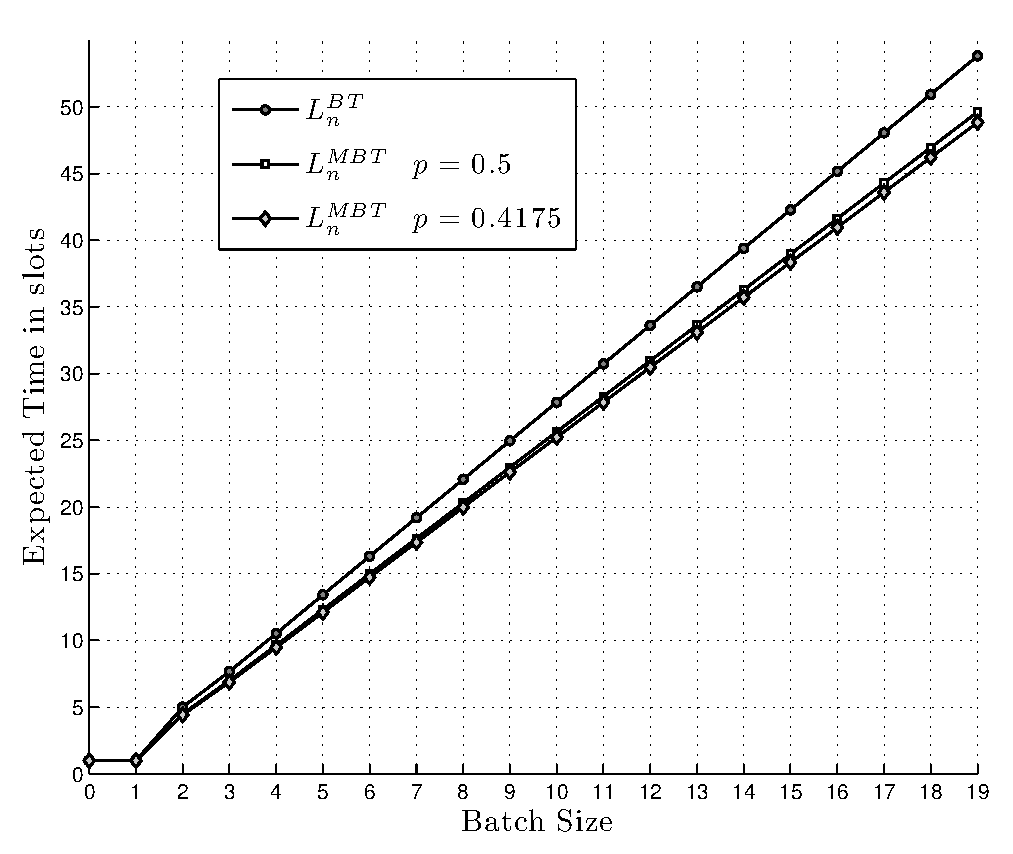
\includegraphics[width=0.7\textwidth]{matlab/BTs/bin-trees-expected-time}
\caption[Expected cost for tree algorithms in \emph{slotted-ALOHA} scenario]{The plot illustrates the expected cost in slots to solve batches of size $n=0,1,\ldots,19$ in a \emph{slotted} Aloha-like scenario using all the basic variants of the tree based algorithms: BT, MBT with sub-optimal $p=0.5$, MBT with optimal $p=0.4175$. All the algorithms show the same behavior: almost linear grow for large $n$. Best performance are provided by MBT with optimal $p$.}
\label{fig:BTs performances}
\end{center}
\end{figure}

Considering the efficiency $\eta_{n}=n/L_{n}^{BT}$ (number of resolved nodes over slots) we have a decreasing series $\eta_{1}=1$, $\eta_{2}=0.40$, $\eta_{3}=0.3913$, \dots, $\eta_{16}=0.3542$ , \dots, $\eta_{31}=0.3505$. It can be shown \cite{capetanakis} that $\eta_{\infty} \approx 0.347$.\\

Since the algorithm is much more efficient in solving small rather than large batches we would prefer to have (ideally)  $n$ batches of size 1 rather than 1 batch of size $n$.\\
Hence, knowing exactly the cardinality $n$ of the initial batch $\mathcal{B}$, we can split the nodes into small groups, of approximately 1 node each, and resolve them faster. \\This is the idea behind many improvements over the basic BT and it reveals the importance of having an accurate estimate of $n$ to efficiently solve a batch.

\begin{comment}
\begin{figure}
\centering
\begin{tikzpicture}[level/.style={->,thick,level distance = 20mm, sibling distance=40mm/#1}]

\node [circle,draw] (z) {$-,2$}
  {child{node [circle,draw] (a) {0,2} edge from parent
            node[ sloped, above, pos=.6] {$Q_{0}(2)$}}
  child {node [circle,draw] (b) {1,1} edge from parent
            node[ right, pos=.6] {$Q_{1}(2)$}}
  child {node [circle,draw] (c) {2,0}{child [grow=up]{node {} edge from parent [draw=none]}} edge from parent
            node[ sloped, above, pos=.6] {$Q_{2}(2)$}}
};
\end{tikzpicture}
\caption[\emph{BT}: Batch split probabilities]{Transaction probabilities to split a set of 2 elements into two sets with $i$, $j$ elements}
\end{figure}
\end{comment}

\subsubsection{Example}

\begin{figure}[htbp!]
\centering
\ovalbox{
\begin{tikzpicture}[level/.style={thick,level distance = 17mm, sibling distance=80mm/#1}]

\node [circle,draw,label=below:\itshape C,label=above:$\epsilon$] (r){1}{
  	child{node [circle,draw,label=below:\itshape C] {2} {
		child{ node [circle,draw,label=below:$n_{1}$] {3} edge from parent node[ above, pos=.5] {0}
			}
		child{ node [circle,draw, label=below:\itshape C] {4}{		
			child{ node [circle,draw,label=below:$n_{2}$] {5} edge from parent node[ above, pos=.6] {0}}
			child{ node [circle,draw,label=below:$n_{3}$] {6} edge from parent node[ above, pos=.6] {1}}
			} edge from parent node[ above, pos=.5] {1}}
			} edge from parent node[above, pos=.5] {0}
  		}
  	child {node [circle,draw, label=below:\itshape C] {7}{
		child{ node [circle,draw, label=below:\itshape C] {8}{
			child{ node [circle,draw,label=below:\itshape I ] {9} edge from parent node[ above, pos=.6] {0}}
			child{ node [circle,draw,label=below:\itshape C] (s10){10} {
				child{ node [circle,draw,label=below:$n_{4}$] {11} edge from parent node[ above, pos=.6] {0}}
				child{ node [circle,draw,label=below:$n_{5}$] (s12){12} edge from parent node[above, pos=.6]{1} }
			}edge from parent node[ above, pos=.6] {1}}
		} edge from parent node[ above, pos=.5] {0}}
		child{ node [circle,draw,label=below:\itshape I ] {13} edge from parent node[ above, pos=.5] {1}}
		} edge from parentnode[ above, pos=.5] {1}
	}
	
};
\end{tikzpicture}
}
\caption[\emph{BT}: Basic binary tree example]{An istance of BT algorithm for $n=5$ nodes. The number inside each circle identifies the slot number. The label below identifies the event occurring: \textit{I} for \emph{idle}, \textit{C} for \emph{collision}, $n_{i}$ for resolution of node $i$. 0/1 branches is analogous to head/tail.}.
\label{example-bbt}
\end{figure}

In Figure \ref{example-bbt} we provide an example to further investigate the behavior of the algorithm. We notice that the instance starts with a collision in slot 1. Then nodes $n_{1}$, $n_{2}$, $n_{3}$ decide to proceed with a retransmission while $n_{4}$, $n_{5}$ remain idle. In slot 2 we see another collision, after it $n_{1}$ transmits again while $n_{2}$ and $ n_{3}$ to stay quiet. In slot 3 we have the first resolution, $n_{1}$ successfully send its message and leaves the collision resolution algorithm.\\
We notice that we can know the cardinality of a collision only after it has been fully  resolved. For example we know only after slot 6 that the collision in slot 2 involved 3 nodes.\\

\begin{comment}
\subsubsection{Nodes addresses}

Looking carefully to the tree you can see that each node resolved is characterized by an \emph{address}: the path from the root to node $n_{i}$ gives  a string of bits. For example node $n_{4}$'s address has as prefix 1010. The prefix in this case can be equivalent to the address but, in a more general case, node address can be a longer string. Assuming in fact that node $n_{4}$'s full address is the 8 bit long string 10100010, running the algorithm brings to the discovery of only the first 4 bits since the collision become resolved without requiring further split of the batch and deeper collision tree investigation (collision in level $t$ provokes a split and a deeper investigation in the tree at level $t+1$ and it requires to consider bit $t+1$ of the nodes' addresses).\\
\end{comment}

\subsubsection{Nodes \emph{id} interpretation}
\label{realvalueapproach}
\marginpar{TUTTO RIFATTO}
BRAs require each node to have a \emph{unique id} to solve the batch. Usually the nodes \emph{id}s are random generated at each algorithm run and can be used to identify a node inside the algorithm. 
There are multiple ways to generate that the \emph{id}, such as:
\begin{itemize}
\item flipping a coin on demand after each collision (step-by-step \emph{id} generation),
\item generating a `long enough' random binary string  at the beginning of the algorithm.
\end{itemize}
We do not want to enter in the details of these choices since there is no reason to prefer one method to the others but device technical limitations.\\ 
Now we want to introduce an interesting interpretation of the \emph{id} that will be used later in algorithms such as EBT (Section \ref{se:EBT}) and Cidon (Section \ref{se:cidon}).\\

In general any infinite length binary string $\mathbf{b_{i}}=(b_{i1}b_{i2}b_{i3}\ldots)$, with $b_{ij} \in \{0,1\}$, can be associated to a real number $r_{i} \in [0,1)$ by a bijective map $r$ defined as follows:

\begin{equation}
r_{i}=r(\mathbf{b_{i}})=\sum_{j=1}^{\infty} \ \frac{b_{ij}}{2^{j}}
\end{equation}
\emph{Each node $n_{i}$ can be associated to a point $r_{i}$ within the real interval [0,1) as well as to the string $\mathbf{b_{i}}$}.\\
For a finite length bit-string $\mathbf{a}=(a_{1}a_{2}\ldots a_{L})$ with length $L=l(\mathbf{a})$ we adapt the definition of $r$ as follows:
\begin{equation}
r(\mathbf{a})=\sum_{j=1}^{L} \ \frac{a_{j}}{2^{j}}
\end{equation}
In this case we have to carry $L$ as auxiliary information to allow the map to remain bijective.\\
Following standard conventions, the empty string $\epsilon$ is prefix of any other string. It has length 0 and $r(\epsilon)=0$.
\begin{comment}
\textcolor{red}{QUESTA OSSERVAZIONE é SOLO FRUTTO DEL MIO SACCO E MI SEMBRAVA INTERESSANTE.\\
An interesting observation is that the distribution of the nodes into the real interval depends upon $p$, the probability  to obtain 0 or 1 tossing a biased coin.
è interessante perchè per il basic binary tree p ottimo è 0.5 per cui si ottiene una distribuzione sperabilmente uniforme dei nodi (o poisson?). Mentre 0.5 non è ottimo per il Modified binary tree: p ottimo 0.4175. quindi la distribuzione migliore per il MBT è una specie di esponenziale discreta e la profondità dell'albero aumenta più ci si avvicina a 1. Questo è quello che mi dice l'intuizione e non ho visto scritto da nessuna parte (magari sul paper orginale del MBT c'è). per cui il MBT non può essere utilizzato banalmente per fare stime tramite una risoluzione parziale di un qualunque sotto intervallo $[0,x)$ con k nodi poichè $n \neq \frac{k}{x} $ (popovski) a meno che non sia nota la distribuzione dei nodi $f(x) $e si normalizzi per $f(x)$ al posto che $x$. 
NOTA: in popovski pg 295  dicono \emph{To summarize, we can say that without any modification, the BT (or the MBT) algorithm offers a way to estimate the unknown conflict multiplicity}. il che è ok ma solo se MBT usa p=0.5
per cui $f(x)=x$. studiare $f(x,p)$?}
\end{comment}

\subsubsection{Tree traversal rules}
\marginpar{TUTTO RIFATTO}
The duality in the interpretation of nodes' \emph{id}s (bit-strings or real numbers) reflects on the duality of the tree traversal rules.\\
According to the adopted approach, enabled nodes can be specified by:
\begin{itemize}
\item a finite length string $\mathbf{a}$ which matches the path from  the root to the first node in the sub-tree they belong to. In this case $\mathbf{a}$ is a prefix  of the enabled nodes \emph{id}s.
\item the couple $ \big(r(\mathbf{a}),l(\mathbf{a})\big)$ which enables the sub-interval $r(\mathbf{a})\leq x <r(\mathbf{a})+{\displaystyle{\frac{1}{2^{l(\mathbf{a})}}}}$
\end{itemize}

\begin{comment}
\textcolor{red}{
The inquirer must provide feedback about the event in a slot but tree walking can be either explicit or implicit. It is explicit if, with feedback, the reader provides also the address in the root of the currently enabled sub-tree. Otherwise it is said to be implicit and each node compute autonomously the new enabled sub-tree.}\\
\end{comment}

To complete the overview of the algorithm we now intuitively describe the tree visit. The following description uses the bit-string approach since a binary string can be immediately mapped to a path in the tree starting from the root.
We assume, following the standard approach, to visit the tree in pre-order, giving precedence to left sub-trees, conventionally associated to 0 branches.\\
The visit starts from the root which has address $\epsilon$.\\
Let $\mathbf{a}$ be the current enabled string, then the following rules apply:
\begin{itemize}
\item If $\mathbf{a}=\epsilon$ and last the event is  a success or an idle slot then the whole conflict has been resolved;
\item If the last event is a collision then we visit the left child of the current node ($\mathbf{a}0$);
\item If the last event is a success or a collision and $\mathbf{a}_{L}=0$ then we visit the right sibling of the current enabled node ($\mathbf{a}1$);
\item If the last event is a success or a idle slot and $\mathbf{a}_{L}=1$ then we look in the path back to the root for the first node whose sibling has not yet been visited. Since we visit the tree in pre-order the next enabled string will be in the form $\mathbf{a}_{k}1$ with $k<L$.
\end{itemize}

A detailed pseudo-code of an algorithm that implements the rules above (and more) can be found in \cite{popovski}. The \emph{Modified Binary Tree} algorithm presented in next section gets a remarkable performance improvement over BT by adding just one new rule.\\

\begin{comment}
Let $b_{1..k}$, with $b_{i} \in \{0,1\}$, $k \geq0$, be the current enabled $k$-bit prefix and \emph{event} $\in \{I,S,C\}$.\\
The possible cases are: \textcolor{red}{qui incasino un po' le cose con una notazione un po' imprecisa}
\begin{enumerate}[i.]
\item \emph{event} is $C$: no matter about $b_{1..k}$, next enabled interval will be $b_{1..k}0$;
\item \emph{event} is not $C$ and $b_{k}=0$: we successfully resolved the left part of the sub-tree, now we will look for right one. Next enabled prefix will be $b_{1..k-1}1$;
\item \emph{event} is not $C$ and $b_{k}=1$: we completed the  resolution of a left sub-tree, now we will look in the way back to the root for the first right sub-tree still unresolved. Let $t$ be $ \arg\underset{i \in 1..k}{\max}|b_{i}=0$ (or $t\gets 0$ if $b_{1..k}$ having 1 or more 1), in other words the position of the right most 0 in the prefix, if any. The new enabled interval will be $b_{t-1}1$. You can see this rule applied after slot 6 and 12 in the example;
\item termination condition is checking $b_{1..k}=\epsilon$.
\end{enumerate}
\end{comment}

\subsection{Modified Binary Tree}
\label{se:MBT}

Modified binary tree is a simple way to improve the BT algorithm.\\ 
\rev{
To keep the notation simple, we will explain the idea illustrating what happens the first time it is applied. In this case  node $\tau$ is visited in slot $\tau$. This does not holds in general, but explanation would have required to use two different indexed for slots and nodes, and Figure \ref{example-mbt} would have been less immediate to understand.\\}

The observation is that, during the tree traversal, sometimes we know in advance if the next slot will be collided. This happens when, after a collided slot $\tau$, we get an idle slot ($\tau+1$) in the left branch of the binary tree. In this case, visiting the right branch ($\tau+2$), we will certainly get a collision .\\
\rev{In fact, after sensing slot $\tau$ is collided, we know that there are at least 2 nodes in the last visited sub-tree. None of them belongs to the left-branch  of that sub-tree since slot ($\tau+1$) is idle. Consequently they must be in the right branch of the sub-tree, whose enabling will hence result into a collision.
 This collision can be avoided by skipping node ($\tau+2$) and visiting its left-child node in slot ($\tau+2$).\\}

\begin{figure}[htbp!]
\centering
\ovalbox{
\begin{tikzpicture}[scale=1, level/.style={thick,level distance = 17mm, sibling distance=80mm/#1}]

\node [circle,draw,label=below:\itshape C,label=above:$\epsilon$] (r){1}{
  	child{node [circle,draw,label=below:\itshape C] {2} {
		child{ node [circle,draw,label=below:$n_{1}$] {3} edge from parent node[ above, pos=.5] {0}
			}
		child{ node [circle,draw, label=below:\itshape C] {4}{		
			child{ node [circle,draw,label=below:$n_{2}$] {5} edge from parent node[ above, pos=.6] {0}}
			child{ node [circle,draw,label=below:$n_{3}$] {6} edge from parent node[ above, pos=.6] {1}}
			} edge from parent node[ above, pos=.5] {1}}
			} edge from parent node[above, pos=.5] {0}
  		}
  	child {node [circle,draw, label=below:\itshape C] {7}{
		child{ node [circle,draw, label=below:\itshape C] (s8) {8}{
			child{ node [circle,draw,label=below:\itshape I ] (s9){9} edge from parent node[ above, pos=.6] (s89){0}}
			child{ node [circle,draw,blue,label=below:\itshape \textcolor{blue}{C},label=45:\textcolor{blue}{SKIP}] (s10){10} {
				child{ node [circle,draw,label=below:$n_{4}$] (s11){11} edge from parent node[ above, pos=.6] (s1011){0}}
				child{ node [circle,draw,label=below:$n_{5}$] (s12){12} edge from parent node[above, pos=.6]{1} }
			}edge from parent node[ above, pos=.6] {1}}
		} edge from parent node[ above, pos=.5] {0}}
		child{ node [circle,draw,label=below:\itshape I ] {13} edge from parent node[ above, pos=.5] {1}}
		} edge from parent node[ above, pos=.5] {1}
	}	
};
%scale=0.8
%\draw [-latex,blue,thin,dashed] (s9) .. controls ++(46:1.6) and ++(0.5,1.6) .. (s11);
%\draw [-latex,blue,thin,dashed] (s11) to [bend left ](s12);
%scale =1;
\draw [-latex,blue,thin,dashed] (s9) .. controls ++(45:2) and ++(0.5,2) .. (s11);
\draw [-latex,blue,thin,dashed] (s11) to [bend left ](s12);
\end{tikzpicture}
}
\caption[\emph{MBT}: Modified binary tree example]{Same example as in Figure \ref{example-bbt} but using \algname{MBT}: tree structure do not change but node 10 is skipped in the traversal.}
\label{example-mbt}
\end{figure}

Expected time analysis is analogous  to Section \ref{basicbinarytreedescription}. The only difference is that after a collision, if we get an idle slot, we will skip the ``next one'' (saving a slot that would certainly be wasted otherwise). Consequently the expected slot cost is $\left[1 \cdot \bigl(1-Q_{0}(n)\bigr)+ 0\cdot Q_{0}(n)\right]$. Let $L_{n}^{MBT}$ be the expected cost in slots to solve a batch of size $n$ using the MBT Alg., then\\
\begin{equation}
L_{n}^{MBT} = \bigl(1 - Q_{0}(n)\bigr)+\sum_{i=0}^{n} Q_{i}(n) (L_{i}^{MBT}+L_{n-i}^{MBT}),
\end{equation}
with
\begin{equation*}
L_{0}^{MBT} = L_{1}^{MBT}  = 1.
\end{equation*}
\rev{Intuitively in this case, since a higher probability to stay silent reduces the expected slot cost, optimal transmit probability will be no longer equal to one half.} At the same time, reducing the transmit probability will increase the number of (wasted) idle slots. Thus the new optimal probability $p$ will be somewhere in the interval (0,0.5).\\
It can be shown \cite{massey} that the best result is achieved for $p=0.4175$, for which the efficiency is asymptotically equal to $\eta \approx 0.381$. This is  +10\% higher than basic BT.\\
In general we have 
\begin{equation}
L_{n}^{MBT}\leq C \cdot n +1, \qquad \textrm{where} \qquad C=2.623.
\end{equation}
Using probability $p={\displaystyle\frac{1}{2}}$  results, for large $n$, in about 1.6\% peak performance loss  ($C=2.667$), which is a moderate decrease. \rev{ It is important to notice that  $p=0.4175$ is close to the optimal bias for small $n$ as well.\\}

\subsection{Clipped Modified Binary Tree}
In this section we will show that, in some cases, partial resolution algorithms can achieve higher efficiency than complete resolution algorithms.\\
The \emph{Clipped Modified Binary Tree (CMBT)} is an adaptation of the \emph{CBT} (see Section \ref{cbt-estimation}) algorithm for complete batch resolution. CBT is like the MBT Alg. but it ends up after two consecutive successful transmissions. Each CBT execution resolves at least two nodes but eventually the last run. Hence, since the multiplicity of the batch to resolve decreases of at least two units after each run, the algorithm terminates for sure.\\

\noindent Collisions tree visit is defined by the following rules: 
\begin{itemize}
\item If the last  run of the CBT does not resolves completely the left sub-tree of the current root, then the next CBT starts from the same root;
\item If the last run of the CBT resolves completely the left sub-tree of the current root, next CBT run is applied to the right child of the current root, that will be considered the new root;
\item While current root left child is \emph{idle}, set the root to the current root right child.
\end{itemize}
Applying the CBT starting each time from the current root makes the algorithm memoryless: its behavior is not affected by previous algorithm runs but the trivial root update. In fact, the root update allows to skip sure collisions and empty slots associated to already resolved sub-sets.\\ 

Efficiency in solving very small batches is CMBT most interesting propriety. This is a consequence of being memoryless. 
Figures \ref{fig:cmbt-vs-mbt} shows how in the average case, the CMBT performs better than the MBT  for batch sizes smaller then 5. Nonetheless, for bigger batch sizes, MBT performs better than CMBT. The gap between the two algorithms gets bigger and bigger as the batch size increases.\\

Consequently, using CMBT is a good idea when the cardinality of the batch to solve is less than or equal to 5 with very high probability.
\begin{figure}[H]
  \begin{center}		         
  \subfloat[\emph{CMBT vs MBT}: very small sizes]{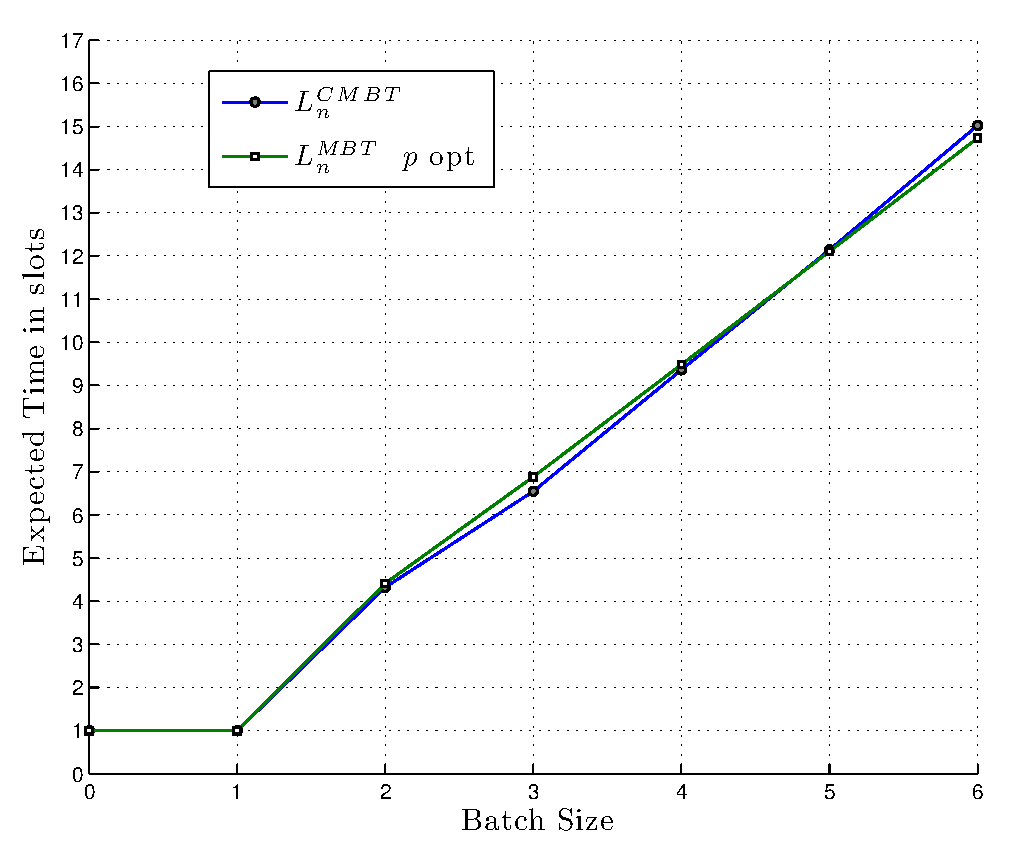
\includegraphics[scale=0.5]{matlab/EBT/CMBT-vs-MBT-small}} 
  \subfloat[\emph{CMBT vs MBT}: larger sizes]{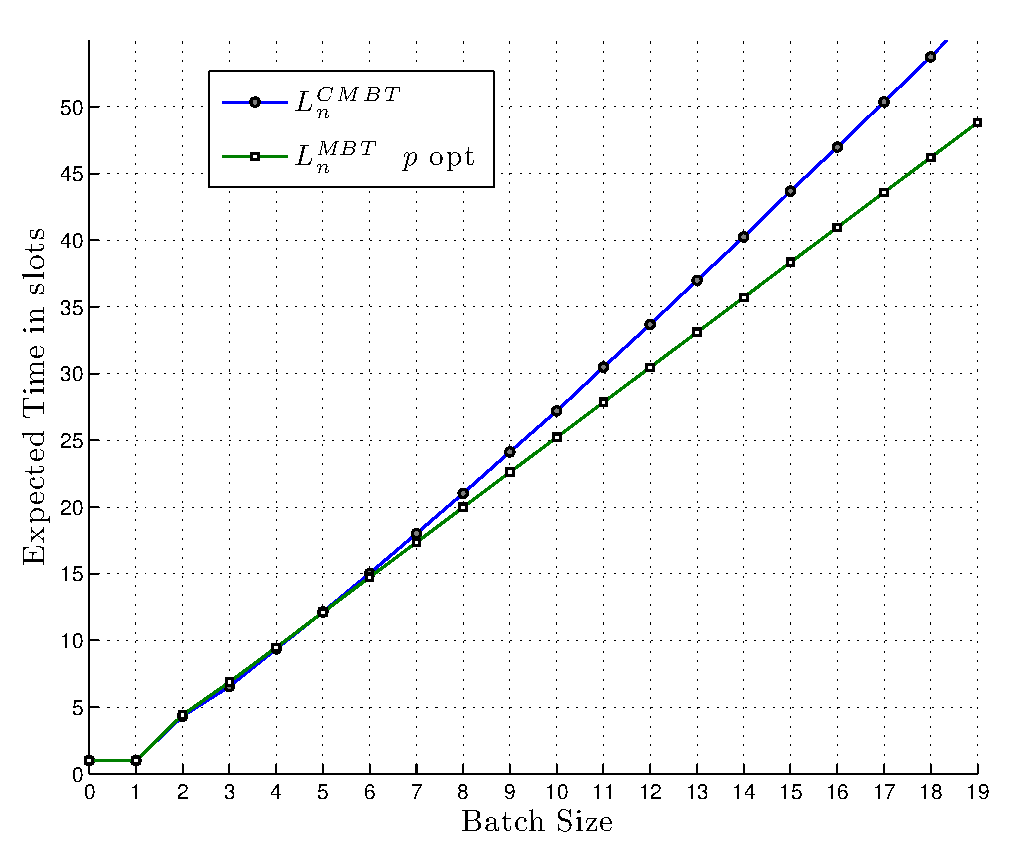
\includegraphics[scale=0.5]{matlab/EBT/CMBT-vs-MBT-large}} 
  \end{center}
\caption[\emph{CMBT} vs \emph{MBT}] {Performance Comparison between CMBT and MBT: the focus is on the expected cost in slots of the \emph{CMBT}  and the \emph{MBT}  algorithms for small sizes. CMBT expected cost was experimentally obtained by running the algorithm on \numprint{10000} random generated instances.} 
\label{fig:cmbt-vs-mbt}   
\end{figure}

CMBT is used by the EBT Algorithm (following Section \ref{se:EBT}) to speed up the resolution.

\begin{comment}
\begin{figure}[H]
\begin{center}
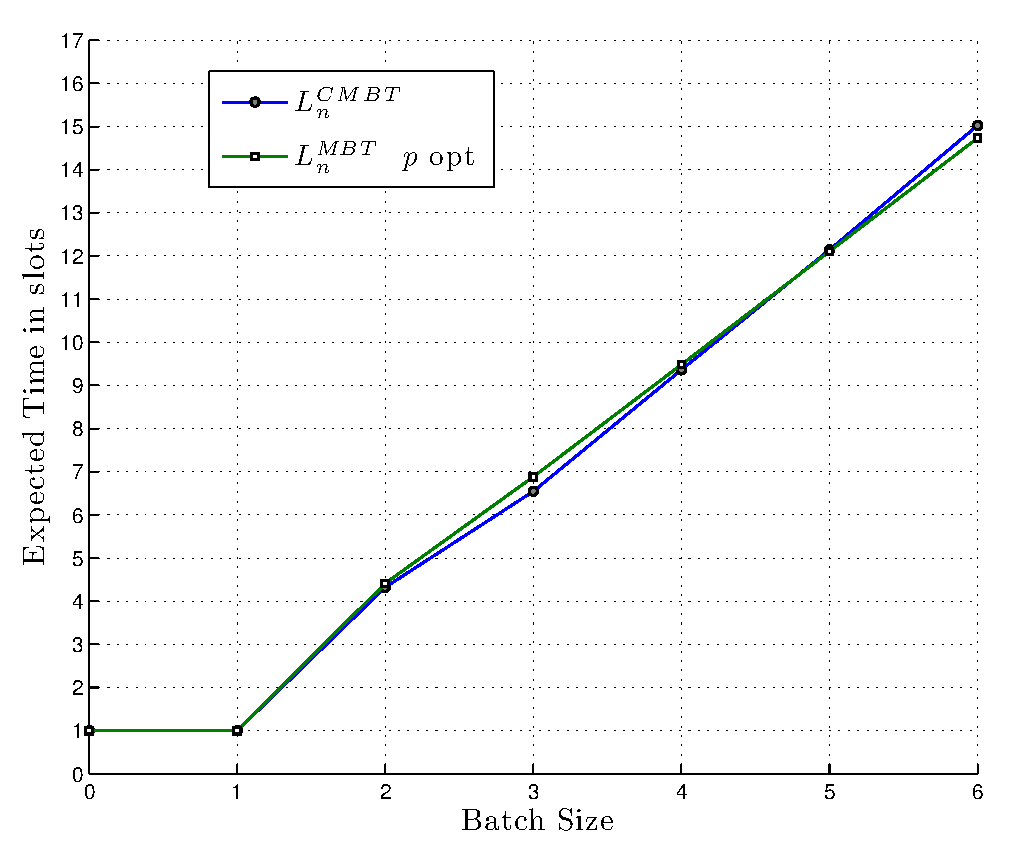
\includegraphics[scale=0.7]{matlab/EBT/CMBT-vs-MBT-small}
\caption{}
\end{center}
\end{figure}

\begin{figure}[H]
\begin{center}
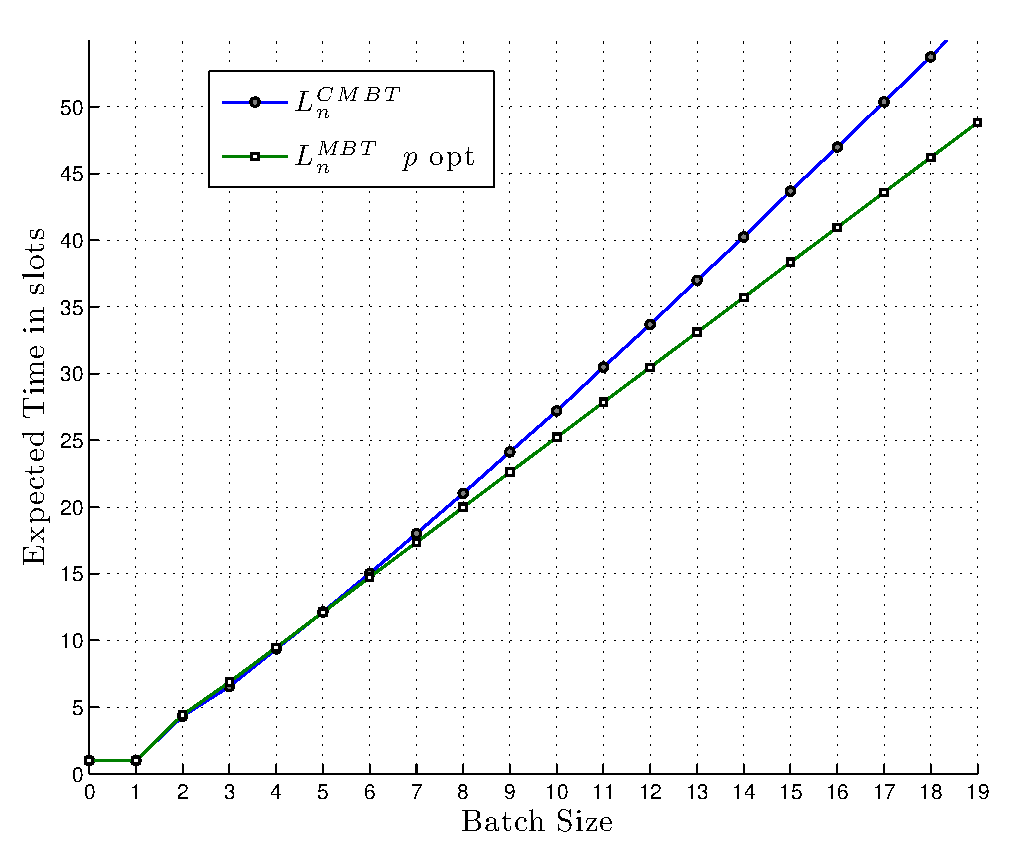
\includegraphics[scale=0.7]{matlab/EBT/CMBT-vs-MBT-large}
\caption{}
\end{center}
\end{figure}
\end{comment}

\subsection{\emph{m} Groups Tree Resolution}
\label{se:mgroups}
\marginpar{NUOVA}

More advanced algorithms for batch resolution, such as those presented in \cite{cidon} and \cite{greenberg87}, share a common idea: divide the initial batch into $m$ groups. We will not deal here about the details of the algorithms and the different approaches  they use to choose $m$. Instead we will concentrate on the common part of these algorithms: divide a batch of size $n$ into $m$ groups and apply a BRA to each group.\\
Given $m$ groups, the probability to have exactly $i$ among $n$ nodes in a group is given by
\begin{equation}
{n \choose i} \left(\frac{1}{m}\right)^{i} \left(1-\frac{1}{m}\right)^{n-i}.
\end{equation}
Let $L_{k}$ be the expected cost to solve a batch of size $k$ with a chosen BRA. Then the expected cost to solve a batch of size $n$ dividing it into $m$ groups is given by
\begin{equation}
\label{eq:BT+m-group-ALOHA}
L'_{n}(\rho)=m \sum_{i=0}^{n}L_{i}{n \choose i} \left(\frac{1}{m}\right)^{i} \left(1-\frac{1}{m}\right)^{n-i},
\end{equation}
where $\rho={\displaystyle\frac{n}{m}}$ is the expected number of nodes in a group.\\

\noindent Figure \ref{m-groups-MBT-ALOHA} shows the results obtained computing  \eqref{eq:BT+m-group-ALOHA} for some batch sizes $n$ varying $\rho$.


\begin{figure}[H]
\begin{center}
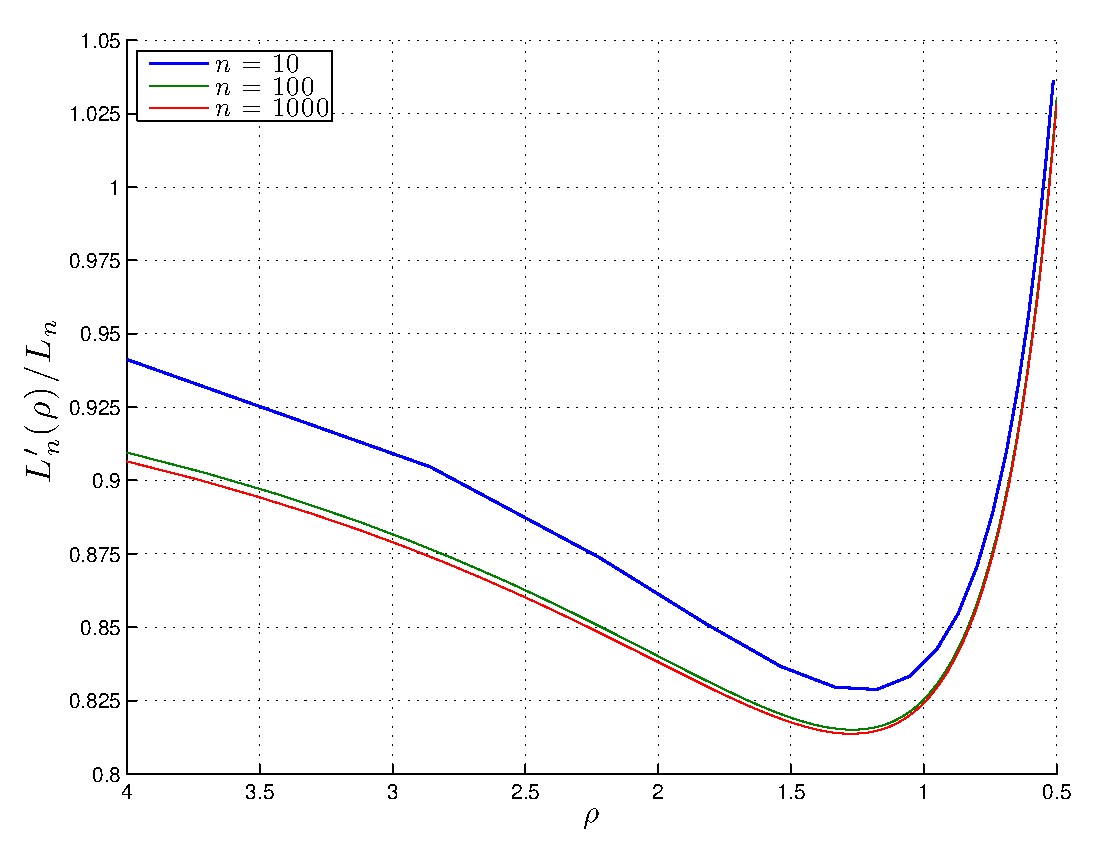
\includegraphics[width=0.7\textwidth]{matlab/BTs/m-groups-MBT-ALOHA}
\caption[$m$ groups split: ALOHA scenario]{\emph{$m$ groups split: ALOHA scenario}. Results were obtained using MBT with optimal probability $p$ in a slotted ALOHA scenario. Splitting the batch into groups provides better results than applying a BRA to the original batch size when $y$-axis values are below 1.}
\label{m-groups-MBT-ALOHA}
\end{center}
\end{figure}

Figure \ref{m-groups-MBT-ALOHA} shows that  $\rho\approx 1.26$ provides the best achievable performance. Furthermore we notice how the knowledge of the batch size is critical: $m$ can be set to the optimal value only knowing exactly the batch size $n$ but often we only have an estimate of $n$. If the estimate is smaller than $n$, performances smoothly degrade but still remain always better than the trivial application of the BRA. On the other hand overestimating $n$ can lead to performance loss when $\rho \approx 0.5$ or smaller.\\

\marginpar{RICHIEDO VERIFICA PER CMSA...\\ $\leftarrow$}
In a CSMA scenario the performances depends on $\beta$ and on the ratio between the nodes packet size ($S_{n}$) and the supervisor feedback size ($S_{f}$). Figure \ref{m-groups-MBT-CSMA} was obtained considering $\displaystyle\frac{S_{n}}{S_{f}}\approx4$. We notice that in CSMA increasing idle slots probability ($\rho$ small) can lower the expected cost. CSMA is also much more robust to an overestimate of $n$ than \emph{slotted}-ALOHA.

\begin{figure}[H]
\begin{center}
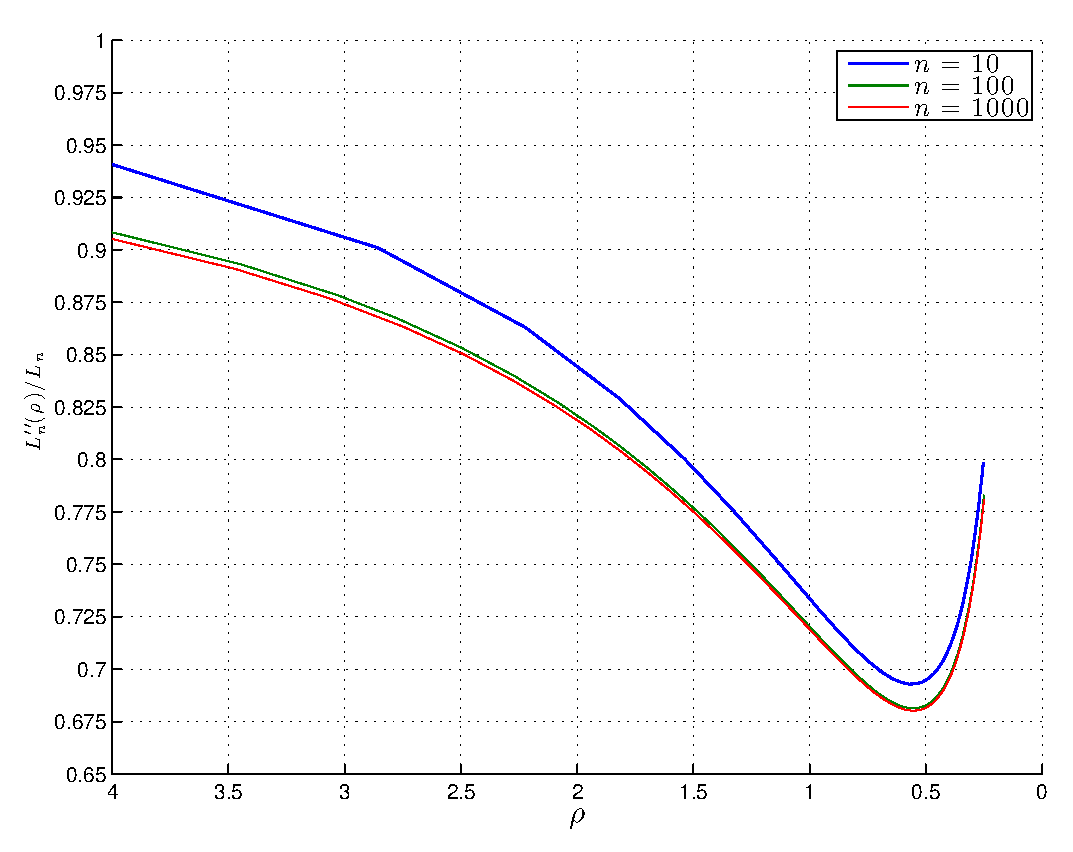
\includegraphics[width=0.7\textwidth]{matlab/BTs/m-groups-MBT-CSMA}
\caption[$m$ groups split: CSMA scenario]{\emph{$m$ groups split: CSMA scenario}. Results were obtained using MBT with optimal probability $p$ in a slotted CSMA scenario. CSMA is more robust to inaccurate estimate than ALOHA.}
\label{m-groups-MBT-CSMA}
\end{center}
\end{figure}


\subsection{Estimating Binary Tree}
\label{se:EBT}
\marginpar{NUOVA}
\emph{Estimating Binary Tree} (EBT) has been recently proposed in \cite{popovski}. It does not work on parameters optimization but tries to use simple heuristics to skip tree nodes that will result in collisions with high probability.\\
Given a batch of size $n$, the keys to understand EBT are the following:
\begin{itemize}
\item in the luckiest scenario running BT results in a balanced binary tree where all the leaves are at the same level,
\item consequently it seems to be a good idea to assume that nodes at levels in the tree less than $\lfloor \log_{2}n\rfloor$ will likely result in collided slots.
\end{itemize}

EBT tries to skip inner nodes of the tree by visiting only nodes at levels equal or deeper than $\lfloor \log_{2}n\rfloor$. Since $n$ is not \emph{apriori} known, a dynamic estimating technique is adopted. To effectively use this estimate tecnique each node must be able to generate values from the standard uniform distribution on the interval [0,1) and to use that value as its unique \emph{id}.\\
 Assume that there are $k$ nodes whose \emph{id}s are in the sub-interval [0,$\pc$) and that they have been previously resolved: all and only the nodes with \emph{id} less than $\pc$ successfully transmitted their messages.  Let $\hat{n}$ express the estimate of $n$. When $\pc$ is greater than 0, setting $\hat{n}$ to $\displaystyle\frac{k}{\pc}$ provides a good estimate of $n$ that becomes more and more accurate as the algorithm goes on. EBT uses $\hat{n}$ (as soon as it is available) to choose the right level in the tree to analyze.\\
 
 The most straightforward  interpretation of the EBT algorithm can be:
 \begin{enumerate}
\item Run the CBT algorithm.
\item Repeat until the end of the process the following steps:
\begin{enumerate}[a)]
\item Update the estimate $\hat{n}$,
\item Start a new CMBT at the next node from level $\lfloor\log_{2}\hat{n}\rfloor$.

\end{enumerate}

\end{enumerate}

Here we gave only a short insight about the algorithm and the estimate technique. In particular this estimate technique is a dynamic adaptation of that described later in Section \ref{se:cidon} and originally proposed in \cite{cidon}.\\

\begin{comment}
\subsection{EBT combined with optimum MBT (DA BUTTARE)}

In this section we describe an improvement over EBT we developed.\\
EBT assumes the nodes to be uniformly distributed in the interval [0,1): this means that their \emph{id} is generated flipping a fair coin. This is a necessary condition for the collision tree to be balanced (the expected height of each leaf is the same) and allows to estimate the level in the tree to analyze using $\lfloor\log_{2}\hat{n}\rfloor$.\\ We remember also that the optimal probability $p$ that provides the best performance  for the MBT is $p=0.4175$. Nevertheless, when $p$ is optimum, the recursive splitting of the original set into 2 subsets, whose expected size is $np$ and $n(1-p)$, returns an unbalanced collision tree.\\ 

\noindent The ideas are the following: 
\begin{itemize}
\item Initially nodes \emph{id}s are uniformly distributed in the tree,
\item Changing a part of a node \emph{id} is allowed if this doesn't affects the already visited conflicting sets,
\item After a collision takes place in a node at level $\hat{N}=\lfloor\log_{2}\hat{n}\rfloor$, the devices involved in the collision  can be redistributed in the collided domain.
\end{itemize}

Let each node $n_{i}$ to be identified by a $L$-length binary string $\mathbf{b_{i}}=(b_{i1}b_{i2}\ldots b_{iL})$. Applying the MBT we resolve a sub-batch or, otherwise, get a collision. In case of collision each node involved updates its \emph{id} as follows: $\mathbf{b_{i}}=(b_{i1}b_{i2}\ldots b_{i\hat{N}}c_{i1}\ldots c_{i(L-\hat{N})})$ where $c_{ik}=0$ with probability $p=0.4175$ and $c_{ik}=1$ with probability $1-p$.\\  

\noindent This modified version of EBT can be briefly described as follows:
 \begin{enumerate}
\item Run the CBT algorithm;
\item Repeat until the end of the process the following steps:
\begin{enumerate}[a)]
\item Update the estimate $\hat{n}$;
\item Start a new MBT at the next node at level $\lfloor\log_{2}\hat{n}\rfloor$ and perform only the first transmission;
\item If the transmission results in a collision, colliding nodes regenerate their \emph{id};
\item Continue  with the current MBT.
\end{enumerate}
\end{enumerate}

\begin{figure}[htb]
\begin{center}
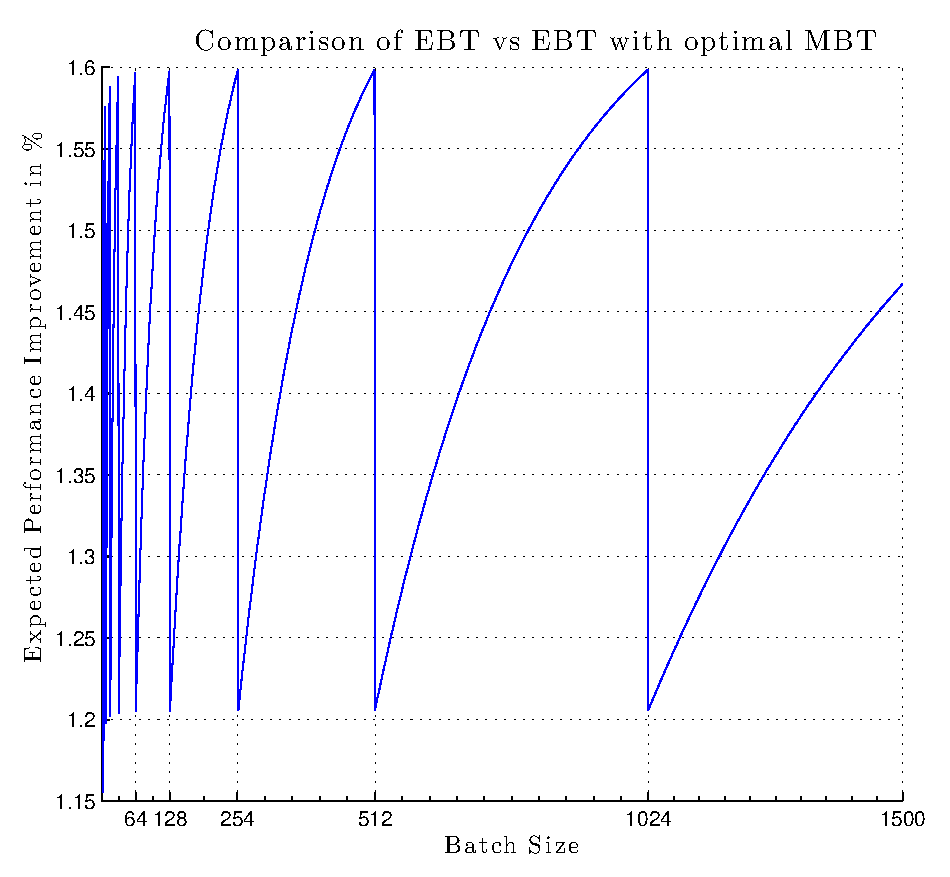
\includegraphics[scale=0.7]{matlab/BTs/EBT-EBT_MBT-Comparison}
\caption[\emph{EBT} vs \emph{EBT with optimal MBT} Performance Comparison]{EBT with optimal MBT provides a minimum expected performance improvement over EBT of 1.2\% and 1.42\% in mean.}
\label{EBTvsEBTopt}
\end{center}
\end{figure}

Figure \ref{EBTvsEBTopt} shows the expected improvement in percentage between  the EBT and the modified EBT algorithm in terms of expected cost ratio. Performance gain results oscillatory with mean 1.42.\\

The \emph{EBT using optimum MBT Algorithm}, proposed in this work, is the average case best \emph{tree-based algorithm with implicit estimate} known so far.

\end{comment}

\section{Others}
In this section we will shortly describe non \emph{tree-based} algorithms for batch resolution.
\subsection{IERC}\marginpar{NUOVA}
The \emph{Interval Estimation Conflict Resolution (IERC)} \cite{popovski} is an adaptation of the FCFS \cite{gallager} algorithm for Poisson's arrivals of packets to the batch resolution.\\
FCFS is the fastest known algorithm to solve Poisson's arrivals and it achieves efficiency $\eta=0.4871$.
It assumes \emph{apriori} knowledge of the arrival rate $\lambda$ of the packets and works by splitting the time in epochs of length $\tau$.\\
Now we briefly describe FCFS Alg. and then we will show how it can be translated to the batch resolution problem.\\ 

At any time $k$, let $T (k)$ be the start time of the current enabled allocation interval. By default, packets generated in the enabled window $(T(k),T(k)+\tau]$ are allowed to be transmitted.
When an \emph{idle} or \emph{successful} event occurs enabled time window gets incremented (shifted towards current time) by $\tau$. On the other hand, if a \emph{collision} takes place, a \emph{Clipped Binary Tree} (see Section \ref{cbt-estimation}) Alg. is started. Assume that CBT resolved the sub-interval $(T(k),T(k)+\alpha(k)]$, then at time $k'$ next FCFS enabled window will be $(T(k'),T(k')+\min(\tau,k'-T(k'))]$ where $T(k')=T(k)+\alpha(k)$.\\

It can be shown \cite{gallager} that setting  $\tau={\displaystyle \frac{1.26}{\lambda}}$ leads to the maximum efficiency. This means that, on average, there are 1.26 nodes in an allocation interval of length $\tau$.\\
The batch resolution problem can be adapted to be solve with an FCFS-like strategy in the following way:
\begin{itemize}
\item nodes \emph{tokens} can be interpreted as arrival times;
\item nodes must be splitted into $m={\displaystyle \frac{n}{1.26}}$ groups so that in each group we expect to have 1.26 nodes;
\item behave FCFS-like to solve the problem.
\end{itemize}
Following  these ideas, IERC achieves the same efficiency $\eta=0.4871$ of FCFS to solve the \emph{Batch Resolution Problem}.

\subsection{Window Based Approaches}
\textcolor{red}{solo per dire che esistono, magari qualche riferimento bibliografico...\\}

\marginpar{NUOVA, RICHIEDO VERIFICA DEL CONTENUTO}
Another possible approach to the batch resolution is to consider a \emph{framed}-ALOHA-like scenario.\\
In \emph{framed}-ALOHA, a frame (alias \emph{window}) is a sequence of consecutive slots.  When a node in the collision batch decides to transmit, it uniformly picks one and only one slot in the window and transmits in that slot.\\
In windows based scenario usually we can work on the optimization of two parameters: $m$, the length of the window in slots, and $p$, the probability that a node transmits in the current window.
Innovate approaches to the problem uses hybrid transmission scheme working by cycles that tries to optimize operational parameters after each transmission windows. On very inexpensive devices usually only windows based algorithms can be implemented.


\chapter{Batch Size Estimate Techniques}
\label{ch:Batch Size Estimate Techniques}
We present here some noteworthy techniques for batch size estimate that can be found in literature.
If a technique was not already identified by a name or associated to a acronym we used the name of one the authors as reference.\\

In general, we assume to have no \emph{a priori} statistical knowledge about the conflict multiplicity. Estimation techniques are thus required to provide accurate estimates for the general zero-knowledge scenario.\\
\section{Clipped Binary Tree}
\label{cbt-estimation}
A simple way to obtain an estimate of the batch size is to solve a minimum number of nodes. This can be done, for example, by using deterministic algorithms such as \emph{Clipped Binary Tree Algorithm} (CBT).\\
CBT is a partial resolution algorithm since only a fraction of the packets of the batch are successfully transmitted.
The algorithm is identical to the MBT (with $\displaystyle p=\frac{1}{2}$ since we require the nodes to be uniformly distributed in the interval [0,1) ) except that it is stopped (the tree is clipped) whenever two consecutive successful transmissions follow a conflict.\\
When the algorithm stops, we know than the last two resolved nodes belong to the same level $i$ of the tree (root is assumed to be at level 0).\\
Therefore, an estimate of the initial batch size is given by:
\begin{equation}
\hat{n}\gets2^{i}
\end{equation}
\begin{comment}
The idea is interesting but the fact of considering recursively subsets of subsets of the initial batch brings to disastrous performance: as reported in \cite{greenberg87}, second and all higher moments of this estimate are infinite.\\
So this simple method is not good to obtain an estimate. 
\end{comment}

\begin{figure}[H]
\centering
\ovalbox{
\begin{tikzpicture}[level/.style={thick,level distance = 17mm, sibling distance=80mm/#1}]

\node [circle,draw,label=below:\itshape C,label=above:$\epsilon$] (r){1}{
  	child{node [circle,draw,label=below:\itshape C] {2} {
		child{ node [circle,draw,label=below:$n_{1}$] {3} edge from parent node[ above, pos=.5] {0}
			}
		child{ node [circle,draw, label=below:\itshape C] {4}{		
			child{ node [circle,draw,label=below:$n_{2}$] {5} edge from parent node[ above, pos=.6] {0}}
			child{ node [circle,draw,label=below:$n_{3}$] {6} edge from parent node[ above, pos=.6] {1}}
			} edge from parent node[ above, pos=.5] {1}}
			} edge from parent node[above, pos=.5] {0}
  		}
	child {node {} {child {node {} edge from parent[draw=none]} child {node {} edge from parent[draw=none]}}edge from parent[draw=none]}
};
\end{tikzpicture}
}
\caption[\emph{CBT}: example]{ Same example as in Figure \ref{example-bbt} but resolution using CBT ends up after two consecutive successful transmissions.}
\end{figure}

Experimental results show that the variance of this obtained estimate is extremely high and the resulting accuracy is really poor.\\ 
This is due to the fact that the batch of interest we use for the estimate becomes, at each level, smaller and smaller: the estimate, even for huge sizes, depends only on very few (3-5) nodes (those at the most left in the tree). Consequently estimate is quite inacurate.\\
Results are reported in Appendix in tables  \ref{CBT-table-1}. Notice how slowly the distribution probability decrease.
\section{Cidon}
\label{se:cidon}
Cidon and Sidi proposed this approach in \cite{cidon}. In their work they describe a complete resolution algorithm based on two phases:
 
\begin{enumerate}
\item Estimating the initial batch size using a partial deterministic resolution scheme. 
\item Performing an optimized complete deterministic resolution based on the results of phase 1. 
\end{enumerate}

The strategy adopted to obtain the estimate is to resolve a small part of the initial batch and to accumulate the number of successful transmissions resulting.\\

A node either takes part to the estimate phase or to the following resolution phase but not both.
The probability $\pc$, which is an algorithm input parameter, determines this choice.
We called it $\pc$ to underlined than this initial choice reflects on the expected accuracy of the resulting estimate.\\

As usual we consider a batch $\mathcal{B}$ of unknown size $n$.
At the beginning of the algorithm each node chooses to transmit with probability $\pc$. Thus the $n$ nodes are partitioned into two set $\mathcal{E}$ and $\mathcal{D}$, where $\mathcal{E}$ consist of those that transmitted and $\mathcal{D}$ the rest. Clearly, $|\mathcal{E}|+|\mathcal{D}|=n$. If the resulting slot is empty or contains a successful transmission, we conclude that $|\mathcal{E}|=0$  or $|\mathcal{E}|=1$, respectively. When a conflict occurs ( $|\mathcal{E}|\geq2$), a complete batch resolution algorithm is started to resolve the conflicts among  the nodes in $\mathcal{E}$ . By simply accumulating in $j$, during the estimate phase, the number of resolved nodes, we know the exact value of $|\mathcal{E}|$.
Then we simply compute our estimate $\hat{n}$ as: 

\begin{equation}
\hat{n} \gets \frac{j}{\pc}.
\end{equation}
When the nodes are uniformly distributed in the real interval [0,1), $\displaystyle \frac{j}{\pc}$  identifies also the expect nodes density in the interval [0, 1) and the nodes in $\mathcal{E}$ are those whose \emph{id} can be mapped to a value belonging to the sub-interval [0, $\pc$).\\
Following Figure \ref{cidon-nodes-id} shows the case providing a simple example.
\begin{figure}[H]
    \centering
    \ovalbox{
    \begin{tikzpicture}
    \draw [thick, [-)] (0,0) node[label=below:0] {}-- (10,0) node[label=below:1] {};
    
    \foreach \x / \y in{1/$n_{1}$,2/$n_{2}$,3.5/$n_{3}$,4/$n_{4}$,5.5/$n_{5}$,7.6/$n_{6}$,9.2/$n_{7}$}
    \draw[->] (\x,1) node [label=above:\y]{} -- (\x,0.3);
    
    % 
    \draw[->] (3,-1) node [label=below:$<\pc\leq$]{} -- (3,-0.3);
    \draw[snake=crosses, very thick] (3,0) node [label=above:0.3] {}-- (3.2,0);
    
    \end{tikzpicture}
    }
    \caption[\emph{Cidon}: initial split]{In this example $\pc=0.3$. At the beginning of the algorithm each node generates its own \emph{id} from the standard uniform distribution on the interval [0,1). Nodes whose \emph{id} is less than $\pc$ owns to $\mathcal{E}$. Nodes whose \emph{id} is greater or equal to $\pc$ owns to $\mathcal{D}$. Estimate of the batch returns $\lceil 2/0.3\rceil=7$ which, in this case, is the exact size of the batch.}
    \label{cidon-nodes-id}
\end{figure}

After the first phase,  the nodes in $\mathcal{E}$ are resolved, but those in $\mathcal{D}$ not yet. To speedup their resolution we are interested in the estimate $\hat{k}$ of $|\mathcal{D}|$, which we can compute as:

\begin{equation}
\hat{k} \gets  \frac{j}{\pc}(1-\pc).
\end{equation}

Then the resolution of $\mathcal{D}$ begins. We note that $|\mathcal{E}| = 0$ does not imply $|\mathcal{D}| = 0$ and consequently a complete resolution algorithm has always to be performed on $\mathcal{D}$.
 
 \begin{algorithm}[h!]
\begin{algorithmic}[1]
	\REQUIRE $\mathcal{B}$ batch with $|\mathcal{B}|=n$
	\REQUIRE $\pc$, fraction of the whole batch to solve
	\STATE \COMMENT{Phase 1}
	\STATE each node flips a coin getting 0 with probability $\pc$, 1 otherwise
	\STATE $\mathcal{E} \,\gets$ \{ nodes that flipped 0\}
	\STATE $\mathcal{D} \gets$ \{ nodes that flipped 1\}
	\STATE \algname{Complete collision resolution ($\mathcal{E}$) }
	\STATE  $\hat{k} \gets |\mathcal{E}|/\pc$
	\STATE \COMMENT{Phase 2}
	\STATE \algname{Optimized complete collision resolution ($\mathcal{D}$,$\hat{k}$, $\pc$) }
	\end{algorithmic}
\caption{\algname{Cidon($\mathcal{B}$, $\pc$)}}
\label{alg-cidon}
\end{algorithm}
 High level peudo-code of \emph{Cidon} algorithm is presented in Alg. \ref{alg-cidon}.\\ \algname{Complete collision resolution ($\mathcal{E}$) } identifies any procedure able to resolve all the nodes in $\mathcal{E}$ allowing them to successfully transmit their messages.\\ \algname{Optimized complete collision resolution ($\mathcal{D}$,$\hat{k}$, $\pc$) } identifies an optimized way to resolve the batch $\mathcal{D}$: the speedup is allowed by the knowledge of its expected multiplicity.\\
 
 The original paper proposes to use an \emph{$m$ groups split} (Section \ref{se:mgroups}) approach to resolve $\mathcal{D}$ where 
 \begin{equation}
m = \max(1, \lceil\alpha \hat{k}-\beta\rceil),
\end{equation}

and each group is resolved by applying the MBT algorithm.\\
The parameter $\alpha$ determines the number of groups, and therefore the efficiency, when $n$ is large, while $\beta$  reduces the number of groups when $n$ is small: many of them would be empty resulting in a waste of time. 
 
 $\alpha=0.786$ determines $\rho\approx 1.27$ which is the \emph{unique} optimum  nodes per group density. $\beta$ and $\pc$ depends on operational requirements: setting $\beta=8$ and  $\pc=0.1$ showed to be a good compromise to get efficient resolution for a wide range of batch sizes.\\  
 
Expected  cost of the estimate phase depends on the BRA used but in general can be considered $O(\pc n)$: time is linear in the size of $\mathcal{E}$.

\subsection{Estimate accuracy}
\label{cidon-estimate-accuracy}

In the original paper \cite{cidon} there is no detailed analysis of the behavior of the estimate algorithm but it is only shown the following fact: as $n$ grows the estimator becomes more accurate.\\
    
Let $J$ be an integer random variable which expresses the number of nodes in $\mathcal{E}$. Given a batch of size $n$, $J$ is binomially distributed with parameter $\pc$. It can be thought as the probability distribution to put $j$ among  $n$ nodes in two bins choosing with probability $\pc$ the first one and $1-\pc$ the other one.  Therefore, we have the following:

\begin{equation}
	P(J=j|n)={n \choose j}\pc^{j}(1-\pc)^{n-j},
           \label{cidon-J}
\end{equation}

\begin{equation}
E[J|n]=n\pc ,
\label{cidon-e-estimate}
\end{equation}

\begin{equation}
\textrm{var}(J|n)=n\pc(1-\pc).
\end{equation}


By applying Chebychev's Inequality \eqref{eq:cheby},  we have for any $\epsilon>0$
 
 \begin{equation}
P\Bigl( \left| J-n\pc\right| \geq \epsilon n \,|\, n \Bigr) \leq \frac{\pc(1-\pc)}{\epsilon^{2}n}.
\label{eq:cidon-cheby}
 \end{equation}
 
 Let $\hat{N}={\displaystyle \frac{\hat{J}}{\pc}}$ be a real-valued random variable that expresses our estimate of $n$. Then from the aforementioned equations \eqref{cidon-J} - \eqref{eq:cidon-cheby} follows that:

\begin{equation}
P\left(\hat{N}=n|n\right)={n \choose j}\pc^{j}(1-\pc)^{n-j} \quad \textrm{with} \quad \hat{n}=j/\pc, \quad 0\leq j\leq n,
\end{equation}

\begin{equation}
E[\hat{N}|n]=n,
\end{equation}
and, finally,
 \begin{equation}
P\left( \left| \frac{\hat{N}}{n}-1\right| \geq \epsilon  \,\big|\, n \right) \leq \frac{1-\pc}{\epsilon^{2}n\pc}.
 \end{equation}
which shows that in this estimation method we can trade off the accuracy with the consumption of resources, time or messages.

\section{Greenberg}


\emph{Basic Greenberg algorithm} strategy is to search for \emph{a power of 2} that is close to $n$ with high probability.\\
The probabilistic test is defined to look for $\hat{n}$ which tries to satisfy:\\
\begin{equation}
\hat{n}\geq 2^{i} \approx n
\end{equation}
Let each of the $n$ conflicting stations either transmit or not transmit in accordance with whether the outcome of a biased binary coin is 0 or 1. The coin is biased to turn up 0 with probability  $2^{-i}$ and 1 with complementary probability. Since the expected number of transmitters is $2^{-i}n$, having a conflict as event supports the hypothesis that $n\geq2^{i}$.\\
Using this test repeatedly with $i=1, 2, 3, \ldots$, leads to the Greenberg \emph{base 2 estimation algorithm}.\\
Each of the conflicting stations executes Algorithm (\ref{alg-greenberg}), resulting in a string of collisions whose lenght determines $\hat{n}$.\\

The probability that at most one node transmits monotonically grows and approaches 1 extremely rapidly as $i$ increases past $\log_{2}n$. Consequently, we expect $i$ is close to $\log_{2}n$.\\

\begin{algorithm}[H]
\begin{algorithmic}
\STATE \COMMENT Each node performs these operations
\STATE $i\gets 0$
\REPEAT
	\STATE $i\gets i+1$
	\STATE choose to transmit with probability $2^{-i}$
\UNTIL {no collision occurs}
\STATE $\hat{n} \gets 2^{i}$
\end{algorithmic}
\caption{\algname{Basic Greenberg ($\mathcal{B}$)}}
\label{alg-greenberg}
\end{algorithm}

The idea behind algorithm \ref{alg-greenberg} appears to be quite simple: as the algorithm goes on the initial unknown batch (of size $n$) is progressively sliced into smaller pieces. Only the nodes virtually inside the enabled slice are allowed to transmit. Slices get thinner and thinner until at most one node is contained in a slice. Figure \ref{fig:greeberg-split} intuitively tries to explain the idea.\\ 

\begin{figure}[htb!]
    \centering
    \begin{tikzpicture}[scale=0.8]  
        \draw (0, 0) circle (3.8cm);
        \foreach \x in {3.5,13.5,...,360}
        \draw[snake=crosses] (\x:3.7) --(\x:3.8);
       \draw[-,ultra thin,dashed] (180:6) to[] (0:6); 
       \draw[-,ultra thin,dashed] (0,0) to[] (-90:6);
       \draw[-,ultra thin,dashed] (0,0) to[] (-135:6);
       \draw[-,ultra thin,dashed] (0,0) to[] (-157.5:6);
       \draw[-,ultra thin,dashed] (0,0) to[] (-168.75:6); 
       \draw[-,ultra thin,dashed] (0,0) to[] (-174.375:6);  
        %arco rosso
        \foreach \x/\text in {1.6,1.7,...,2.5}
        \draw [-,thin,red!50] (0:\x) arc(0:-90:\x);
        %arco  blue
        \foreach \x/\text in {2.6,2.7,...,3.5}
        \draw [-,thin,blue!50] (0:\x) arc(0:180:\x); 
        %arco verde
        \foreach \x/\text in {.6,.7,...,1.5}
        \draw [-,thin,green!80] (-90:\x) arc(-90:-135:\x);

        \draw [<->,ultra thin,blue] (5:5) arc(5:175:5);
        \draw [<->,ultra thin,red] (-5:5.3) arc(-5:-85:5.3);
        \draw [<->,ultra thin,green] (-95:5.6) arc(-95:-130:5.6);
        
        \path[text width=3pt]
        (90:6)      node[above right] {$\pi$}  (95:2)      node[below] {$n/2$}
        (-45:6)      node[below right] {$\pi/2$} (-50:2.7)      node[right] {$n/4$}
        (-112.5:6)      node[below left] {$\pi/4$} (-118:2)      node[below left] {$n/8$};
    \end{tikzpicture}
    \caption[\emph{Basic Greenberg}: batch split idea]{Visually nodes can be thought to be uniformly distributed on the circumference of a circle. By performing Greenberg's algorithm we go and analyze each time a smaller sector (in this case the half of the previous one) of the circle and find when a sector contains only 1 or no nodes.  Not overlapping sectors are drawn to maintain the image simple but in general nodes gets redistributed to each step of the algorithm}
    \label{fig:greeberg-split}
\end{figure}

Expected running time is $O(log_{2}n)$. In particular, since in the \emph{slotted}-ALOHA model considered in the paper reader feedback is supposed to be transmitted at the end of each transmission slot, expected running time can be expressed, in slot numbers, as $\approx 1+\log_{2}n$.\\

An important note is that the algorithm always involves all the nodes in the batch: in each stage of the algorithm each node has to take a choice if transmit or not. 
Each choice is independent of what the node did in the previous steps. \\ 
This is of great importance and allows $\hat{n}$ to have bounded moments: it can be shown for large $n$ that:
\begin{equation}
E[\hat{n}] \approx n\phi,
\end{equation}
\begin{equation}
E[\hat{n}^{2}] \approx n\Phi,
\end{equation}
where
\begin{equation}
\phi= \frac{1}{\log2} \int_{0}^{\infty} \! e^{-x}(1+x) \prod_{k=1}^{\infty}\bigl(1-e^{-2^{k}x}(1+2^{k}x)\bigr)x^{-2} \, dx = 0.91422\dots
\end{equation}

\begin{equation}
\Phi= \frac{1}{\log2} \int_{0}^{\infty} \! e^{-x}(1+x) \prod_{k=1}^{\infty}\bigl(1-e^{-2^{k}x}(1+2^{k}x)\bigr)x^{-3} \, dx =1.23278\dots
\end{equation}

\noindent $\phi$ and $\Phi$ where obtained in \cite{greenberg87} using advanced mathematical analysis supported by Mellin integral transform\footnote{in this work we only report these as final results, please refer to the original paper to see how $\phi$ and $\Phi$ where obtained.}.
In general $\phi$ and $\Phi$ depend on the size of the problem. Following Table \ref{table:phi-Phi} shows the behavior of the expected estimate (and therefore $\phi$) as function of $n$.\\

\begin{table}[H]
\caption[\emph{Basic Greenberg}: Expected Estimate]{Given a batch of size $n$ the expected estimate applying base 2 Greenberg is $E[\hat{n}|n]$. The ratio $E[\hat{n}|n]/n$ monotonically decreases and gets stable at $0.9142$. This shows that this estimate technique provide biased results.}
\begin{center}
\begin{tabular}{rD{.}{.}{5.2}D{.}{.}{1.4}}
\toprule
 n & \multicolumn{1}{r}{$E[\hat{n}|n]$} & \multicolumn{1}{c}{$E[\hat{n}|n]/n$} \\ \midrule
1 &     2.00 &   2.0000 \\ 
2 &     2.56 &   1.2822 \\ 
4 &     4.21 &   1.0533 \\ 
8 &     7.89 &   0.9863 \\ 
16 &  15.20 &   0.9498 \\ 
32 &    29.82 &   0.9320 \\ 
64 &    59.08 &   0.9231 \\ 
128 &   117.59 &   0.9186 \\ 
256 &   234.60 &   0.9164 \\ 
512 &   468.64 &   0.9153 \\ 
1024 &   936.71 &   0.9148 \\ 
2048 &  1872.86 &   0.9145 \\ 
4096 &  3745.14 &   0.9143 \\ 
8192 &  7489.72 &   0.9143 \\ 
16384 & 14978.86 &   0.9142 \\ 
32768 & 29957.16 &   0.9142 \\ 
65536 & 59913.74 &   0.9142 \\\bottomrule
\end{tabular}
\end{center}
\label{table:phi-Phi}
\end{table}
The fact that, for large $n$, $E[\hat{n}] \approx n\phi$ suggests a way for correcting the estimate bias and allows to assume $\hat{n}_{+} = {\displaystyle\frac{\hat{n}}{\phi}}$ as a estimate of n. Owing to the contribution of periodic functions, $\hat{n}_{+}$ is not an asymptotically unbiased estimate of $n$, in the sense that  $E[\hat{n}_{+}]/n$ does not tend to 1 as $n$ gets large. Fortunately, the amplitude of the periodic functions turns out to be less than $2 \cdot10^{-5}$, so this bias is negligible for all practical purposes.\\


Interestingly, a simple variant of the estimation algorithm has provably disastrous performance. Consider the algorithm in which each station involved in the initial collision transmits to he channel with probability $\frac{1}{2}$. If this causes another collision, then those that just transmitted, transmit again with probability $\frac{1}{2}$. The others drop out. This continues, with the stations trying to transmit always being a subset of those that just transmitted, until there is no collision. Take $2^{i}$ as the estimate of the multiplicity of conflict where $i$ is the number of the steps until ther is no collision. It can be shown that the second and all higher moments of this estimate are infinite.

\subsection{Base \emph{b} variant}

Using basic Algorithm \ref{alg-greenberg}, even though the expected value of $\hat{n}_{+}$ is quite close to $n$, $\hat{n}_{+}$ is likely to differ from $n$ by a factor of 2. In the original work a small generalization of the base 2 algorithm is proposed to overcome this limitation: providing an estimate whose mean is  close to $n$ but whose  distribution peaks more sharply about the mean.\\
Simply it is suggested to use $b$ instead of 2 as base, with $1<b\leq2$.\\
\begin{algorithm}[H]
\begin{algorithmic}
\STATE $i\gets 0$
\REPEAT
	\STATE $i\gets i+1$
	\STATE transmit with probability $b^{-i}$
\UNTIL {no collision occurs}
\STATE $\hat{n}(b) \gets 2^{i}$
\STATE $\hat{n}_{+}(b) \gets \hat{n}(b)/\phi(b)$
\end{algorithmic}
\caption{\algname{base \emph{b} Greenberg ($\mathcal{B}$)}}
\label{alg-greenberg-base-b}
\end{algorithm}

$\phi(b)$ corrects the bias of the estimator. $\phi(b)$ is the optimal correction when $n$ is large.
Looking at Table \ref{table:greenberg-b-phi} you can notice how smaller $b$ results in smaller $\phi(b)$. This means that $b$ deeply biases the estimate: if $b^{'} < b^{''}$ then $E[\hat{n}(b^{'})] < E[\hat{n}(b^{''})]$.\\ This is a result of the following fact: let $i^{''}$ be the expected slot the base $b^{''}$ algorithm will end up given a batch size $n$, then $i^{''} \leq log_{b^{''}} n$. Let $i^{'}$ be the same for $b^{'}$. If $b^{'} < b^{''}$ then $b^{'i^{'}} > b^{''i^{''}}$ \symbolfootnote[2]{This comes from experimental observations.}

%nota della tabella, assicurarsi che sia nella stessa pagina

\begin{table}[H]
\caption[\emph{Greenberg}: different $b$ summary]{Following table shows how $\phi$ and ``Expected \emph{Greenberg base b algorithm} cost in slots'' vary for different $b$. Expected cost ($\lesssim \log_{b}n$) is expressed as a multiplicative factor for the basic Greenberg algorithm cost ($\lesssim \log_{2}n$).}
\label{table:greenberg-b-phi}
\begin{center}
\begin{threeparttable}
\begin{tabular}{lccl}
$b$ & $\phi(b)$\tnote{a} &\,\,\,& Expected cost in slots-1\\
\toprule
2          & $\approx 0.9142$ && $\lesssim 1 \qquad\,\,\, \times \log_{2} n$\\
1.1       & $\approx 0.3484$ && $ \lesssim 7.27$\\
1.01     & $\approx 0.1960$ && $ \lesssim 69.66$\\
1.001   & $\approx 0.1348$ && $ \lesssim 693.49$\\
1.0001 & $\approx 0.1027$ && $ \lesssim 6931.81$\\
\bottomrule
\end{tabular}
\begin{tablenotes}
\item [a] {\footnotesize \smaller Code used to compute $\phi(b)$ is provided in Appendix \ref{sec:greenberg-moments}}
\end{tablenotes}
\end{threeparttable}
\end{center}
\end{table}

It can be shown \cite{greenberg87} that, \emph{for all n greater than some constant $n_{0}(b)$}\\
	\begin{equation} 
		\left |\frac{E[\hat{n}_{+}(b)]}{n}-1 \right | < \epsilon(b) ,
	  \end{equation}

\begin{equation}
		\frac{\sigma\bigl(\hat{n}_{+}(b)\bigr)}{n}< \epsilon(b) ,
	\end{equation}

\emph{where $\epsilon(b) \to 0$ as $b \to 1$.}

In other words when $b \to 1$ and $n$ is large the estimate becomes unbiased and variance goes to 0: we have ideally a perfect estimator.\\
Our experimental results showed that this base $b$ estimator is not so good for real life scenarios.  




\section{Window Based}

Windows based approaches use a \emph{framed}-ALOHA-like transmission scheme where the reader provides feedback to the nodes after each frame. \emph{Framed}-ALOHA is characterized by the frame length $L$, whose choice is critical for the performance of the resolution process as well as the estimation phase. In fact, in \emph{framed}-ALOHA there is no clear distinction between resolving the nodes and estimating  their number since the estimate can be performed only by knowing the outcome of the last enabled window.\\
Setting $L$ large compared to the batch size increases the probability to solve all the nodes in the current window but, on the other hand, it leads to an inefficient waste of slots and consequently sub-optimal running time.  At the same time $L$ large provides a very accurate estimate of the batch size.\\
Setting $L$ small leads to collided slots with very high probability. Thus nodes whose transmissions collided have to try again in the next contention windows. Since we don't know how many nodes took part in a collision we can state that collisions provides poor information about the batch multiplicity. More collisions we have, less accurate will be our estimate.\\
Intuitively we can think that setting $L$ equal to the batch size  $n$ is a good choice. In fact it is, but the problem is that we do not know $n$.\\

An interesting approach to the problem is expressed in \cite{lucent}. When the scenario allows to use a \emph{probabilistic-framed-ALOHA}\footnote{\emph{probabilistic-framed-ALOHA} is an extension of the \emph{framed-ALOHA} model where a node takes part to the current contention window with probabily $p$ or waits for the next one with probability $1-p$. Nodes that decide to transmit behave like in the standard \emph{framed-ALOHA}.} scheme we can play with one more parameter: $p$, the probability for a node to take part in the current transmission window. Setting $p$ small allows to keep $L$ small too and hence, when $n$ is large, provides an accurate estimate of the whole batch considering only a sub-set of it. This results in shorter estimate time.\\

Since when $p=1$ \emph{probabilistic-framed-ALOHA} reduces to simple \emph{framed-ALOHA} and it is reasonable to start any estimate algorithm with $p=1$, we will show a possible approach to the problem in a \emph{framed-ALOHA} scenario. \\

Let $n$ be the batch size and $L$ the window length. The probability that $k$ among $n$ nodes choose the same slot is binomially distributed with parameters $B(n,1/L)$. Then the probabilities to get an \emph{idle} slot , a \emph{successful} one or a \emph{collision} are respectively given by:
\begin{equation}
p_{0}(n)=\left(1-\frac{1}{L}\right)^{n}
\end{equation}

\begin{equation}
p_{1}(n)=\frac{n}{L}\left(1-\frac{1}{L}\right)^{n-1}
\end{equation}

\begin{equation}
p_{2+}(n)=1-p_{i}(n)-p_{s}(n)
\end{equation}

Hence we have three possible events, each one associated to its probability. Considering the whole window, the possible outcome of the transmissions consists in a tuple $(i,s,c)$ of  $i$ idle, $s$ successful, $c$ collided slots which satisfies $i+s+c=L$.
Hence, the probability to get $i$ idle slots, $s$ successful transmissions and $c$ collision is given by:

\begin{equation}
P(i,s,c)= \frac{L!}{i!\,s!\,c!} \ p_{0}(n)^{i} \ p_{1}(n)^{s}\ p_{2+}(n)^{c} = \frac{L!}{i!\,s!\,c!} \  \fw(i,s,c,n).
\label{eq:Pisc}
\end{equation}

Once we have tried to resolve the batch using a window approach we know how many idle, successful or collided slots there were.\\ Then we  find the estimate $\hat{n}$ as the batch size that  maximizes the probability to see the tuple $(i,s,c)$ in a $L$ length window:
\begin{equation}
\hat{n}=\argmax_{\displaystyle n} \fw(i,s,c,n),
\end{equation}
where we discarded the factorial terms because they not contribute to identify the maximum since $L$, $i$, $s$, $c$ are fixed. Furthermore, since $L$, $i$, $s$, $c$ are fixed, $\fw(i,s,c,n)$ becomes a one-variable function which results well behaved in $n$, being initially monotonically increasing and then monotonically decreasing. Therefore $\fw(i,s,c,n)$ has only one maximum.

By setting 
\begin{equation}
\fw'(i,s,c,n)=0,
\label{eq:dummy-eq}
\end{equation}
and numerically solving \eqref{eq:dummy-eq} we can obtain the batch size that maximizes our function. In general the solution will not be integer-valued and a rounding operation is necessary to achieve a real world batch estimate.\\
\begin{table}[H]
\centering
\caption[\emph{Window based estimate: Possible estimates when $L=10$}]{Estimate given $(i,c,s)$ when $L=i+c+s =10$.}
\label{tb:window-estimate}
\resizebox{0.5\textwidth}{!}{
\begin{tabular}{|c|c|c|c|c|c|c|c|c|c|c|}
\hline
\backslashbox{$c$}{$s$}&0&1&2&3&4&5&6&7&8&9 \\\hline
1 & 3 & 3 & 4 & 5 & 6 & \multicolumn{1}{r|}{7} & \multicolumn{1}{r|}{8} & \multicolumn{1}{r|}{9} & \multicolumn{1}{r|}{10} &11 \\ \hline
2 & 5 & 6 & 7 & 8 & 8 & \multicolumn{1}{r|}{10} & \multicolumn{1}{r|}{11} & \multicolumn{1}{r|}{12} & \multicolumn{1}{r|}{13} & - \\ \hline
3 & 7 & 8 & 9 & 10 & 11 & \multicolumn{1}{r|}{12} & \multicolumn{1}{r|}{13} & \multicolumn{1}{r|}{14} & - & - \\ \hline
4 & 10 & 11 & 12 & 13 & 14 & \multicolumn{1}{r|}{15} & \multicolumn{1}{r|}{16} & - & - & - \\ \hline
5 & 12 & 14 & 15 & 16 & 17 & \multicolumn{1}{r|}{19} & - & - & - & - \\ \hline
6 & 16 & 17 & 19 & 20 & 22 & - & - & - & - & - \\ \hline
7 & 20 & 22 & 23 & 25 & \multicolumn{1}{l|}{-} & - & - & - & - & - \\ \hline
8 & 26 & 28 & 30 & \multicolumn{1}{l|}{-} & \multicolumn{1}{l|}{-} & - & - & - & - & - \\ \hline
9 & 35 & 38 & \multicolumn{1}{l|}{-} & \multicolumn{1}{l|}{-} & \multicolumn{1}{l|}{-} & - & - & - & - & - \\ \hline
10 & \multicolumn{1}{l|}{$\infty$} & \multicolumn{1}{l|}{-} & \multicolumn{1}{l|}{-} & \multicolumn{1}{l|}{-} & \multicolumn{1}{l|}{-} & - & - & - & - & -\\\hline
\end{tabular}
}
\end{table}

Table \ref{tb:window-estimate} shows the estimate provided by the explained technique when $L=10$. Cells identified by $(c,s)$ where $c+s>10$ cannot be associated to any estimate since their events are impossible. The case $c=0$ is trivial since the estimate is exact and is given by the number of successful transmission.\\
We note also that when we see only collisions, the estimator is not able to provide a finite estimate. The event $c=10$ in the table is in fact associated to $\hat{n}=\infty$. In general, when $c=L$ we have that \eqref{eq:Pisc} reduces to:

\begin{equation}
P(0,0,L)=\ p_{2+}(n)^{L} = \left[1-\left(1-\frac{1}{L}\right)^{n}-\frac{n}{L}\left(1-\frac{1}{L}\right)^{n-1}\right]^{L},
\end{equation}

\noindent which is maximized ($P(0,0,L)=1$) by $n=\infty$ for any $L$. Hence we would not to have only collisions since they do not provide any information about the cardinality of the batch.\\ A larger  window has to be used to get a finite estimate but its optimal length remains unknown.

\chapter{Estimate Performance Analysis}
\label{ch:Performance Analysis}

In the previous Chapter we presented some noteworthy  \emph{batch size estimation  (BSE) algorithms}.\\ Now we would provide the reader a practical overview of the results achieved by each estimation scheme.\\
We will analyze \emph{Cidon} to show which is the minimum amount of nodes to be resolved for the estimate to be within user-required constrains with high probability.\\  
We will analyze the behavior of \emph{Greenberg} when varying the batch size.\\
Finally, we propose and analyze a modification of \emph{Greenberg}, named \emph{Enhached Greenberg Algorithm (EGA)}, which tries to refine the raw estimate provided by the original algorithm.
\section{Cidon BSE}

\begin{equation*}
\end{equation*}
We remember from Section \ref{cidon-estimate-accuracy} that
\begin{equation*}P(J=j|n)={n \choose j}\pc^{j}(1-\pc)^{n-j},\end{equation*}
and
\begin{equation*}\hat{n}=\frac{j}{p}.\end{equation*}
Note that  in Alg. \ref{alg-cidon} (Cidon) we have $\pc$ \emph{a priori} fixed since it is an input parameter of the algorithm. Consequently $J$ is a binomial distribution with parameters $B(n,\pc)$ and recalling \eqref{cidon-e-estimate}
we get:
\begin{equation}
E[\hat{n}|n,\pc]=\frac{1}{\pc}E\left[j|n,\pc\right]=n, \qquad \forall \,\pc
\end{equation}
This shows that Cidon provides an unbiased estimator ($E[\hat{n}|n]=n$) independently from $\pc$: $\pc$ influences only the variance of the estimator. 

\begin{equation}
\begin{split}
\textrm{var}(\hat{n}|n) & =E[\hat{n}^{2}|n]- E[\hat{n}|n]^{2}\\
& = \frac{1}{\pc^{2}}E[j^{2}|n] - n^{2}\\
& = \frac{n\pc(1-\pc)+n^{2}\pc^{2}}{\pc^{2}}- n^{2}\\
& =  \frac{n}{\pc}-n
\end{split}
\end{equation}

\begin{figure}[htbp]
\begin{center}
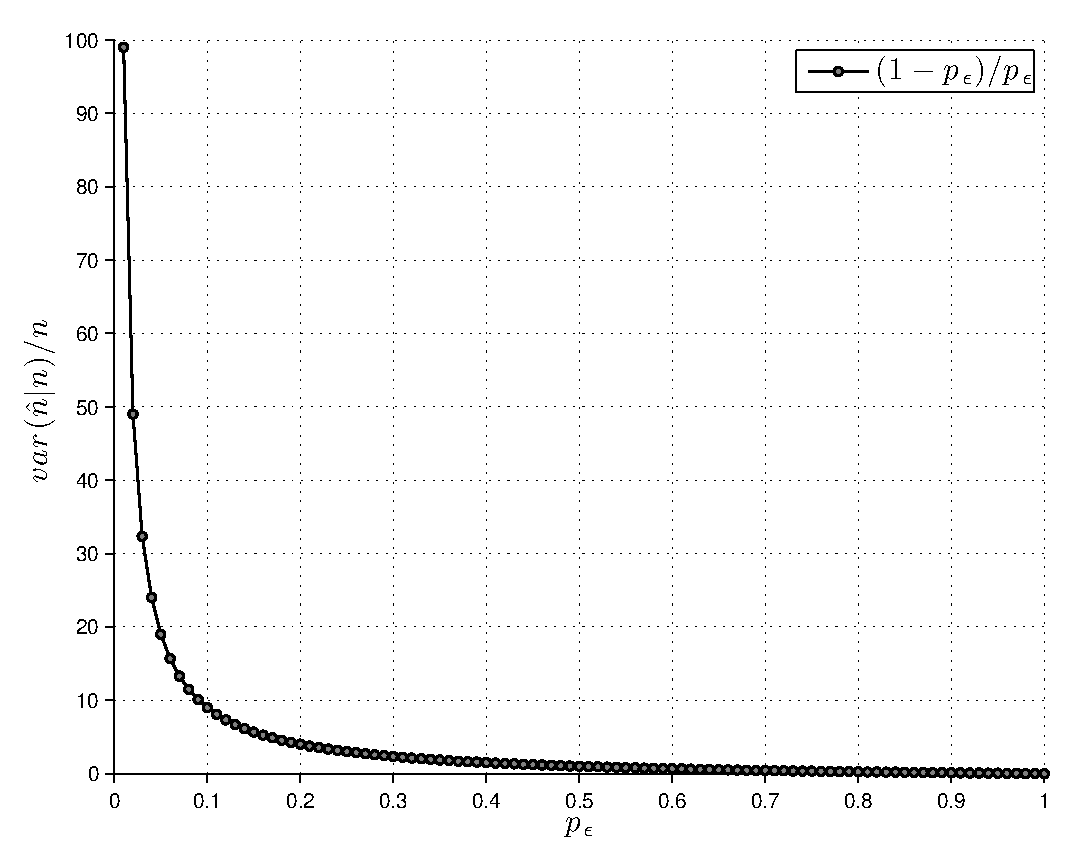
\includegraphics[width=0.7\textwidth]{matlab/Cidon/cidon-variance-p}
%\epsfile{file=matlab/Cidon/cidon-variance-p.eps,scale=0.8}
\caption[\emph{Cidon}: Variance behavior]{\emph{Cidon}:  estimate accuracy dramatically improves while $\pc\leq0.1$.}
\end{center}
\end{figure}

Variance is strict monotonically decreasing in $\pc$.
Anyway it is difficult to establish in what measure an estimate can be considered accurate.\\
Given $n$, let $k \geq1$ define the minimum required accuracy in the following way: 
\begin{equation}
\frac{n}{k}\leq\hat{n}\leq kn
\label{cidon-accuracy-constrains}
\end{equation}
Let $\theta$ be the probability we require for constrains \eqref{cidon-accuracy-constrains} to be satisfied.\\
If we set $\theta=0.99$, we can find the minimum $\pc$, ensuring the estimate to be within confidence interval \eqref{cidon-accuracy-constrains}, by solving the following problem.\\
\begin{equation}
\begin{split}
P\left(\frac{n}{k}\leq \hat{n} \leq kn \big| k,n\right)=& P\left(\frac{n}{k}\leq j/\pc \leq kn \big| k,n,\pc\right)\\
=&P\left(\frac{n\pc}{k}\leq j \leq kn\pc \big| k,n,\pc\right)
\end{split}
\label{cidon-accuracy-bounds}
\end{equation}
Probability in \eqref{cidon-accuracy-bounds} is well behaved and expresses a constrain for $j$, which is a value assumed by $J$ mentioned in \eqref{cidon-J}. Since $J$ assumes positive integer values we introduce rounding operations. In particular, rounding effect is non neglectible when $n\leq 200$.  \\
\begin{equation}
f(k,n,\pc) = P\left(\left\lceil \frac{n\pc}{k}\right\rceil\leq j \leq \left\lfloor kn\pc\right\rfloor \big| k,n,\pc\right)\geq \theta
\end{equation}
Fixed $k$, $n$ and $\theta$, $\pc$ can be found by numerically solving\footnote{in this work we used bisection method}:
\begin{equation}
f(k,n,\pc) = \theta
\end{equation}
Figure below shows minimum $\pc$ in function of $k$ for different batch sizes.\\

\begin{figure}[htbp]
\begin{center}
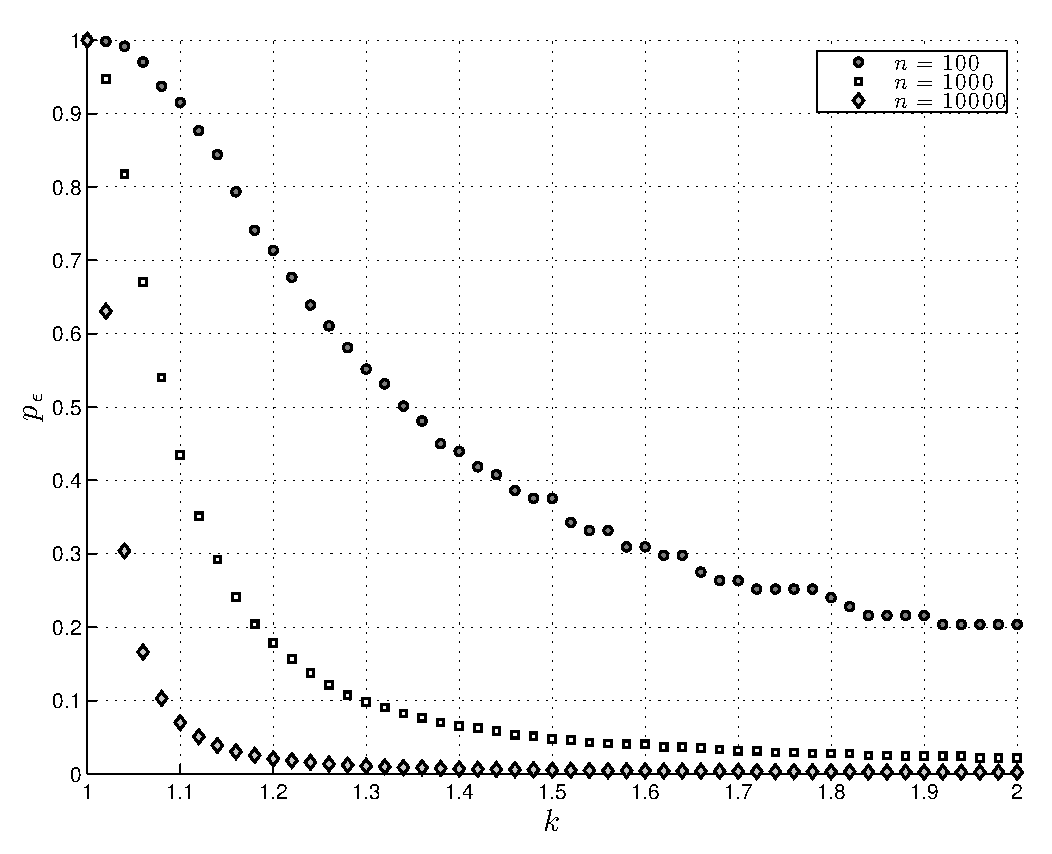
\includegraphics[width=0.7\textwidth]{matlab/Cidon/cidon-k-p-minimum}
\caption[\emph{Cidon}: Minimum $\pc$ required for accuracy  $k$]{\emph{Cidon}: Minimum $\pc$ required for accuracy at least $k$ with $\theta=0.99$, plot step is 0.02}
\label{cidon-k-p-minimum}
\end{center}
\end{figure}

Figure \ref{cidon-k-p-minimum} shows how the fraction of the initial batch to resolve for estimate to be within  required confidence interval with high probability deeply depends on the size of the problem: smaller sizes require much higher $\pc$.\\
At the same time, considering absolute cost in elapsed slots, Figure  \ref{cidon-k-L-minimum} shows that, for a wide range of $k$, the time required is quite independent of the size of the problem.\\
Time required by the largest considered $n$ provides a  bound for smaller ones.\\
Note that in Figure  \ref{cidon-k-L-minimum} an upper bound on the expected BRI time taken is plotted: this bound is not so tight for very small batches. With very small batches tree based BRAs performs better than what is reported.   

\begin{figure}[htb!]
\begin{center}
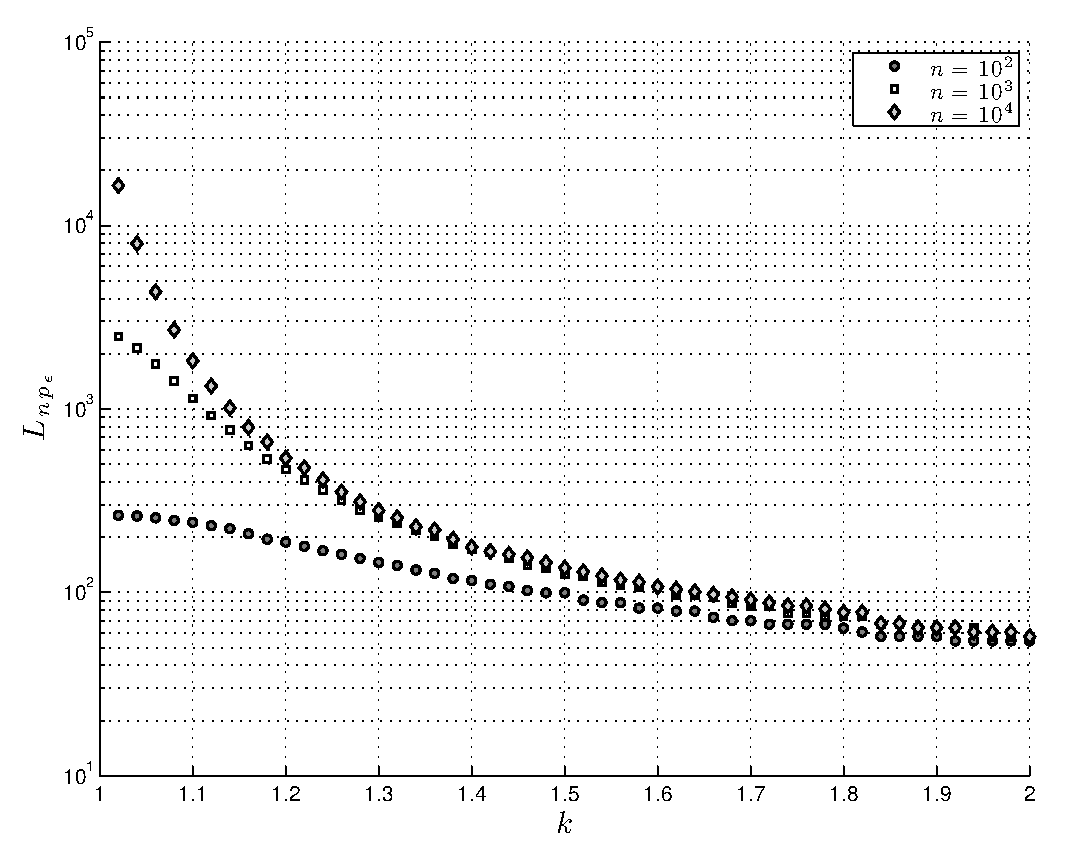
\includegraphics[width=0.7\textwidth]{matlab/Cidon/cidon-k-L-minimum}
\caption[\emph{Cidon}: Upper bounds on the expected time required for accuracy $k$]{\emph{Cidon}: Upper bounds on the expected time (in slots) required to achieve accuracy at least $k$ with $\theta=0.99$,  plot step is 0.02}
\label{cidon-k-L-minimum}
\end{center}
\end{figure}

\section{Greenberg BSE}
Given a current slot transmission probability $p$ and a batch of size $n$ we define respectively:
\begin{enumerate}
\item the probability to get an empty slot (no transmissions)
\begin{equation}q_{0}(p,n)=(1-p)^{n} \label{eq:greenberg-prob-empty}\end{equation}
\item the probability to get a successful transmission (one transmission)
\begin{equation}q_{1}(p,n)=n p (1-p)^{n-1} \label{eq:greenberg-prob-succ}\end{equation} 
\item the probability to get a collision (two or more transmissions)
\begin{equation}q_{2+}(p,n)=1-q_{0}(p,n)-q_{1}(p,n)\label{eq:greenberg-prob-coll}\end{equation}
\end{enumerate}

In basic Greenberg (\emph{Alg.} \ref{alg-greenberg}) each slot is associated with a different probability $p$. Naming each slot $i$ starting with $1, 2, \dots,$ we have:
\begin{equation}
	p_{i}=p(i)=2^{i}
\end{equation}

Given $n$ nodes, the probability to terminate algorithm \ref{alg-greenberg} in slot $i$ is given by:
\begin{equation}
\fg(n,i)=\prod_{k=1}^{i-1}q_{2+}(p_{k},n) \cdot \bigl( q_{0}(p_{i},n)+q_{1}(p_{i},n)\bigr)  
\label{eq:bgstopprobability}
\end{equation}

An overview of the behavior of $\fg(n,i)$ is presented in table \ref{basic-greenberg-stop-probabilities} on page \pageref{basic-greenberg-stop-probabilities}.\\ Equation \eqref{eq:bgstopprobability} defines the probability for biased estimate $\hat{n}$ to be equal to $2^{i}$ when the batch size is $n$. 
\begin{equation}
\textrm{Pr}\left( \hat{n}=2^{i}|n\right)=\fg(n,i)  
\end{equation}

Following Figures \ref{fig:greenberg-dist-small} and \ref{fig:greenberg-dist-large} show how the distribution behaves respectively for small and large sizes.
We note that, for any fixed $n$, the distribution is well behaved: initially it is monotonically increasing, then a monotonically decreasing part follows.\\
It turns out that, for batch sizes larger than 128, the distribution is ``stable'' in the sense that doubling the number of nodes produces a shift of 1 slot to the right but the values assumed are the same (see Figure \ref{fig:greenberg-dist-large} ).\\


\begin{figure}[htbp]
\begin{center}
%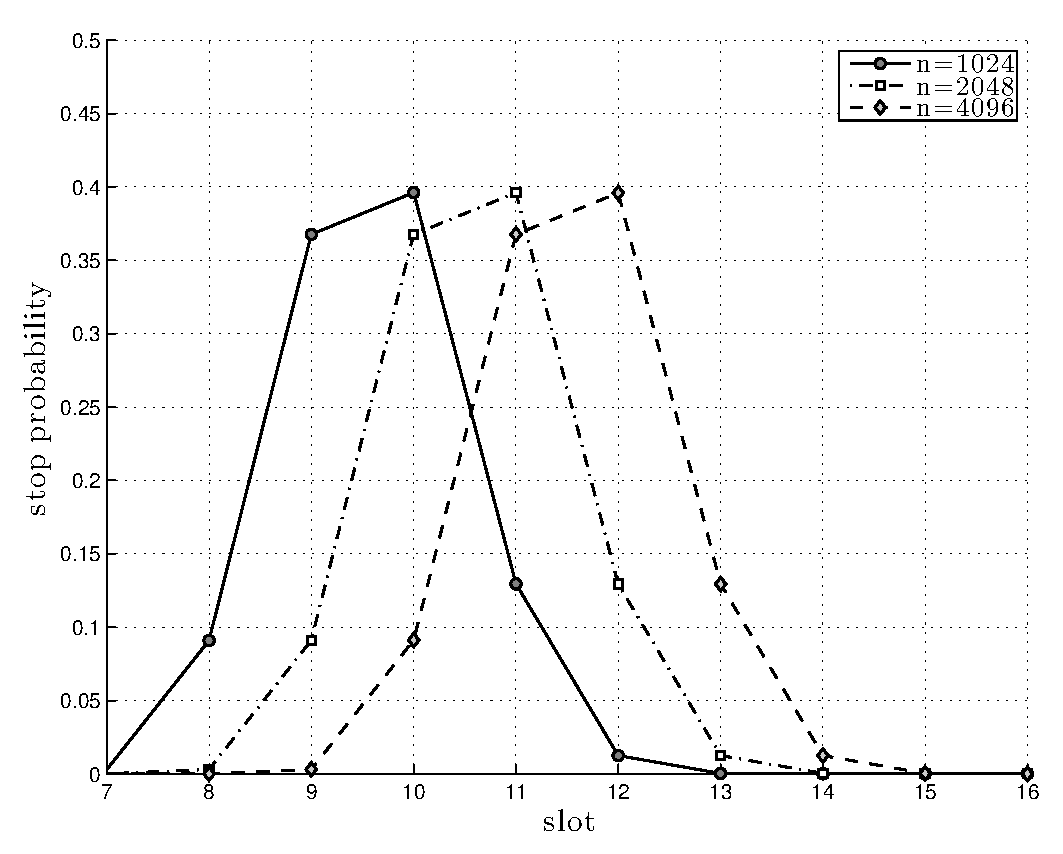
\epsfig{file=matlab/Greenberg_stop_prob/greenberg-stop-distribution-uniformity.eps,scale=0.7}
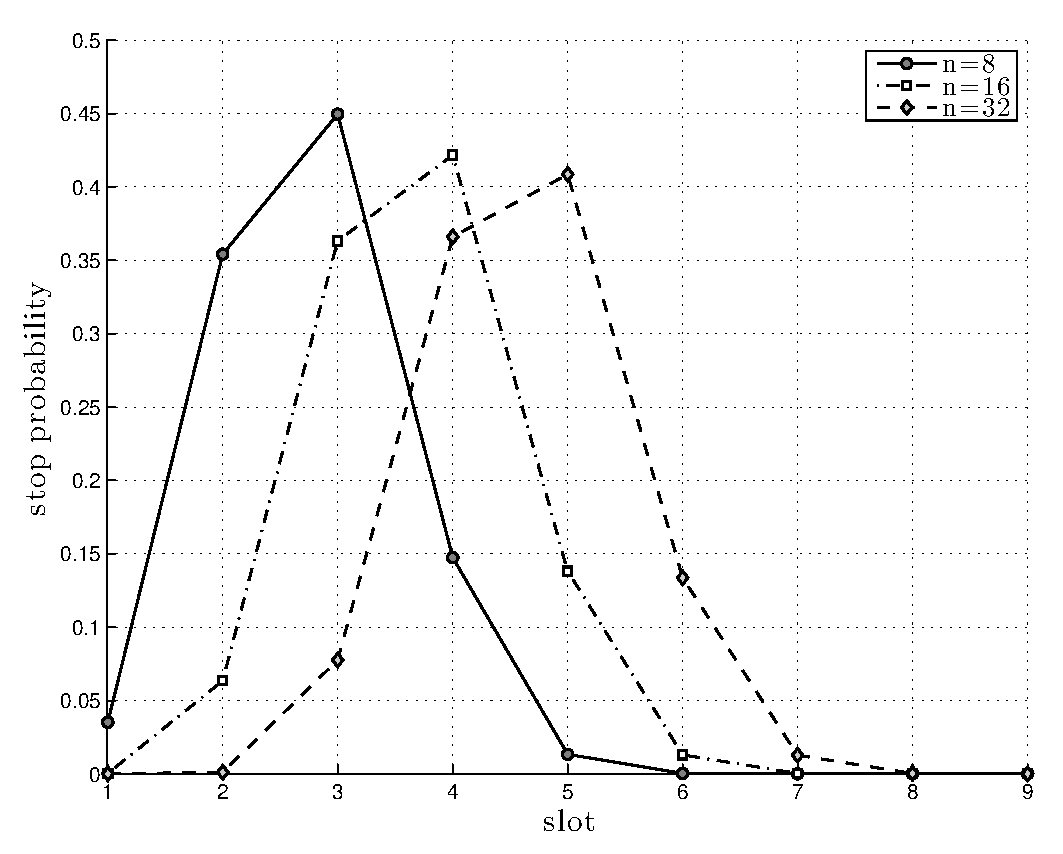
\includegraphics[width=0.7\textwidth]{matlab/Greenberg_stop_prob/greenberg-stop-distribution-uniformity-init}
\caption{\emph{Basic Greenberg}:  small $2^{k}$ sizes distribution.}
\label{fig:greenberg-dist-small}
\end{center}
\end{figure}


\begin{figure}[H]
\begin{center}
%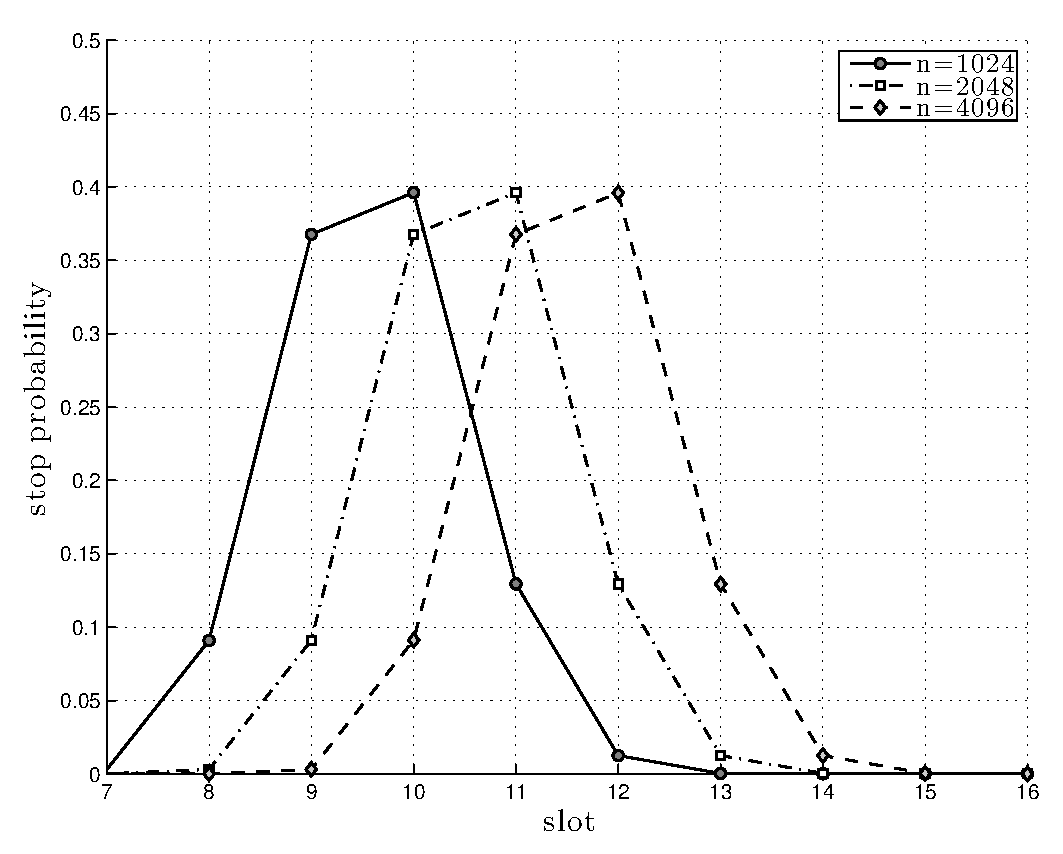
\epsfig{file=matlab/Greenberg_stop_prob/greenberg-stop-distribution-uniformity.eps,scale=0.7}
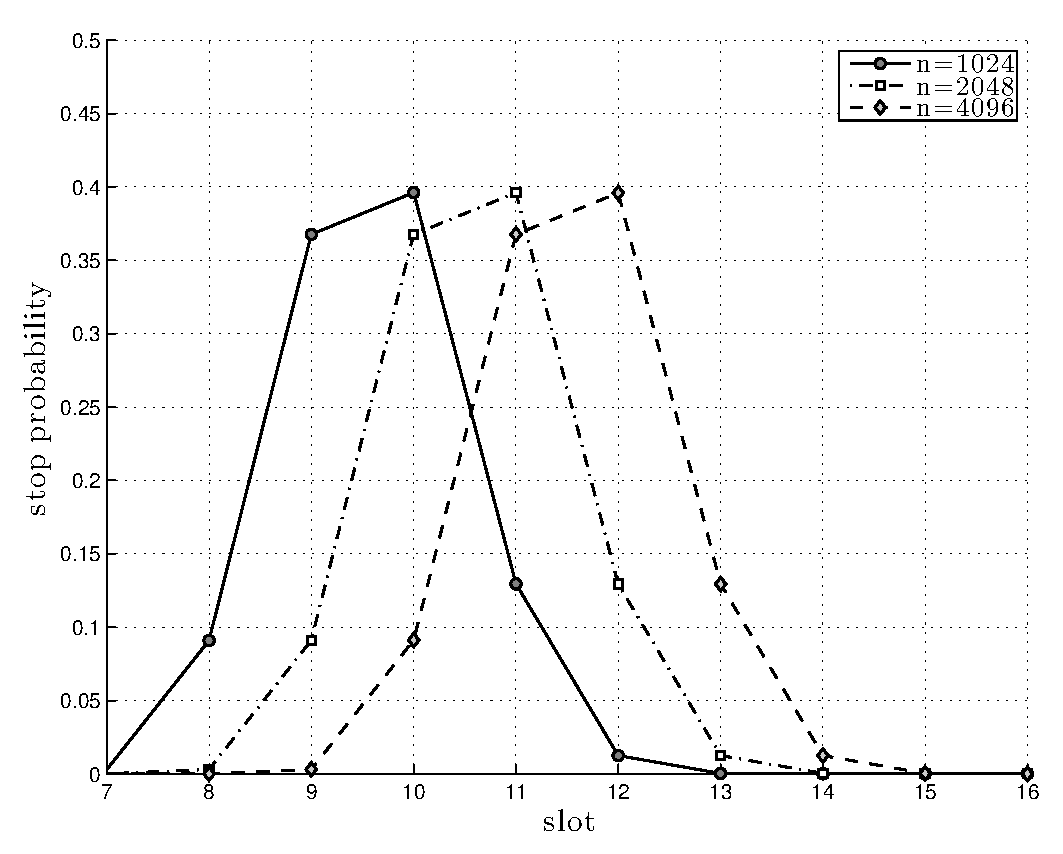
\includegraphics[width=0.7\textwidth]{matlab/Greenberg_stop_prob/greenberg-stop-distribution-uniformity}
\caption{\emph{Basic Greenberg}:  large $2^{k}$ sizes distribution.}
\label{fig:greenberg-dist-large}
\end{center}
\end{figure}


\begin{figure}[H]
\begin{center}
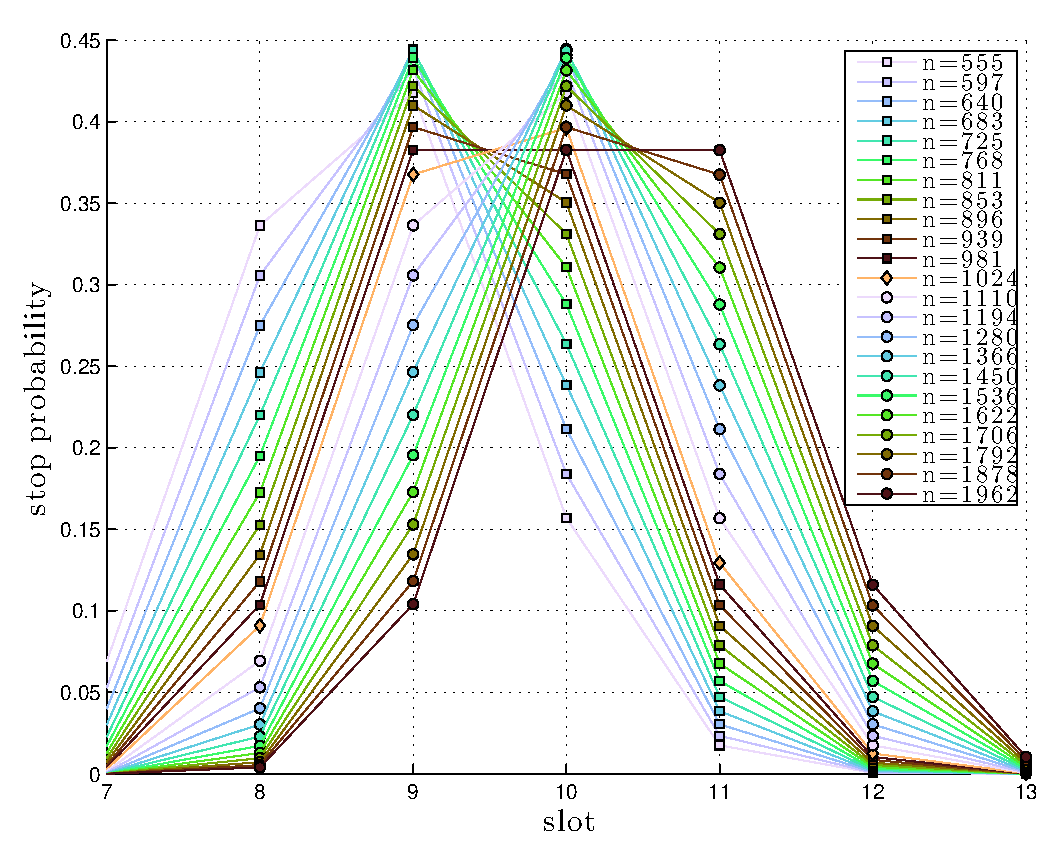
\includegraphics[width=0.7\textwidth]{matlab/Greenberg_stop_prob/greenberg-stop-distribution-intermediate-values}
\caption{\emph{Basic Greenberg}:  general sizes distribution.}
\label{fig:greenberg-dist-general}
\end{center}
\end{figure}
This is not only true for sizes power of two but for any size. Figure \ref{fig:greenberg-dist-general} shows the case where size $n'$ has color $c$ and size $2n'$ has, again, color $c$ but a different marker: values are the same but shifted right. Interestingly the highest peaks are located in $n=683$ and $n=1366$.

%\subsection{Base $b$ Greenberg}
\subsection{Considerations}
Greenberg method is really good from the point view of running cost since it is $O\bigl(\log_{2}n\bigr)$ respect to the size  $n$ of the problem but it has also some non negligible drawbacks:
\begin{enumerate}[\bf a)]
\item estimation phase results in a sequence of colliding messages. These provides informations about the cardinality of the batch but do not help to solve an, even small, portion of the eventually following batch resolution problem and can not carry auxiliary infromations. An algorithm that allows to get an estimate while transmitting successfully messages would offer some advantages when the problem is not only the pure estimation but also a subsequent resolution.
\item it does not allow to achieve arbitrary precision in the estimate.\\ In fact we have that:
	\begin{enumerate}[\it i.]
		\item  the estimate is, by construction, a power of 2. Only a small subset of batch sizes can be mapped without any error.
		\item the end-up distribution is not sharp enough but it spans over a few slots: this is shown by Figure \ref{fig:greenberg-dist-large}. The Figure shows that, for the examined batch sizes, fixed a problem of size $n$ we have about:
		\begin{itemize}
		\item 0.02\textpertenthousand\  estimate is $16n$;
		\item 3\textpertenthousand\  estimate is $8n$;
		\item 1.2\% estimate is $4n$;
		\item 12.9\% estimate is $2n$;
		\item 39.6\% estimate is $n$; $\checkmark$
		\item 36.8\% estimate is $\frac{n}{2}$;
		\item \ 9.1\% estimate is $\frac{n}{4}$;
		\item \  3 \textperthousand\ estimate is $\frac{n}{8}$;
		\item \ 0.02\textpertenthousand\ estimate is $\frac{n}{16}$;
		\end{itemize}
		It is difficult to discriminate between $n$ and $\frac{n}{2}$ 
	\end{enumerate}
\item to get a tighter estimate, base $b$ Greenberg has to be used. Anyway to improve the accuracy very small $b$ has to be used (see Table \ref{table:greenberg-b-phi}) and this results in worse running times: even if theoretically it remains $O(log_{b}n)$ which is a lower order term compared to $n$, in practice estimate time can be no more neglected. In this case, for reasons expressed in {\bf a)}, using Greenberg  could be a bad choice.
\end{enumerate}

\section{EGA BSE}

Let $n$ be a batch size and $p$ be a given transmission probability. As expressed by \eqref{eq:greenberg-prob-empty} \eqref{eq:greenberg-prob-succ} \eqref{eq:greenberg-prob-coll}, varying $n$ while $p$ is fixed results in very different probabilities for \emph{idle}, \emph{successful} and \emph{collided} slots.

\begin{figure}[htbp]
\begin{center}
%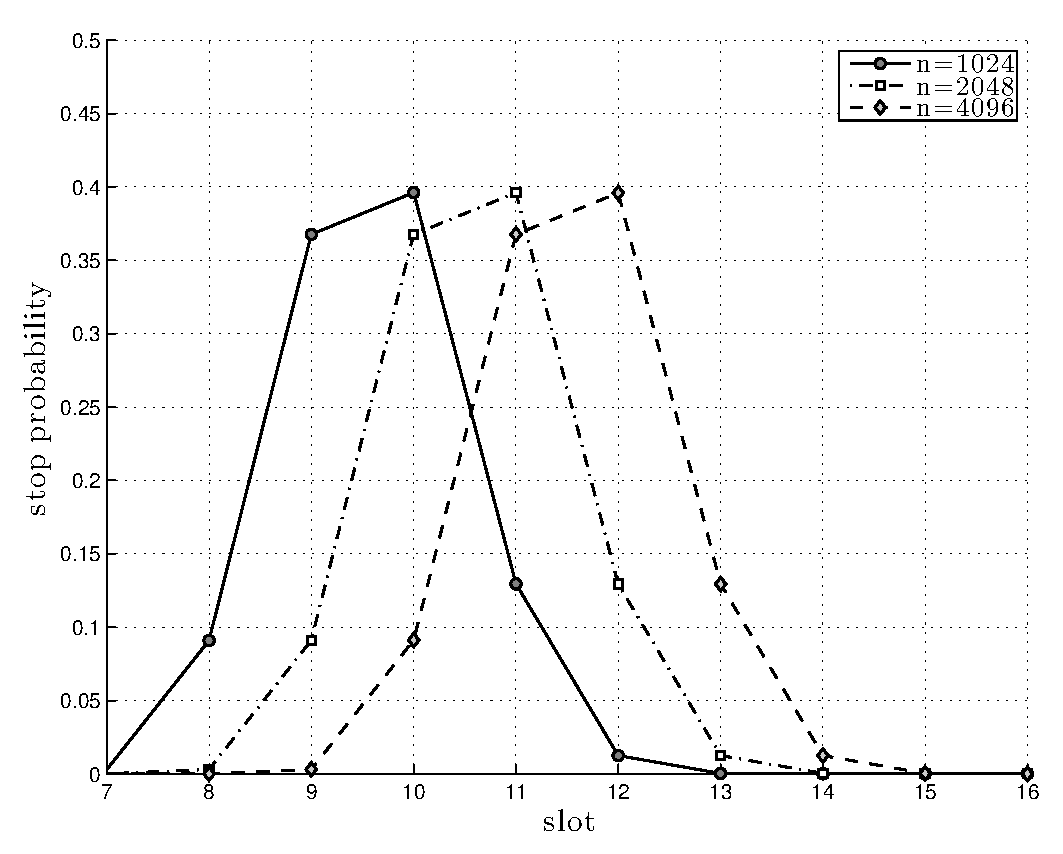
\epsfig{file=matlab/Greenberg_stop_prob/greenberg-stop-distribution-uniformity.eps,scale=0.7}
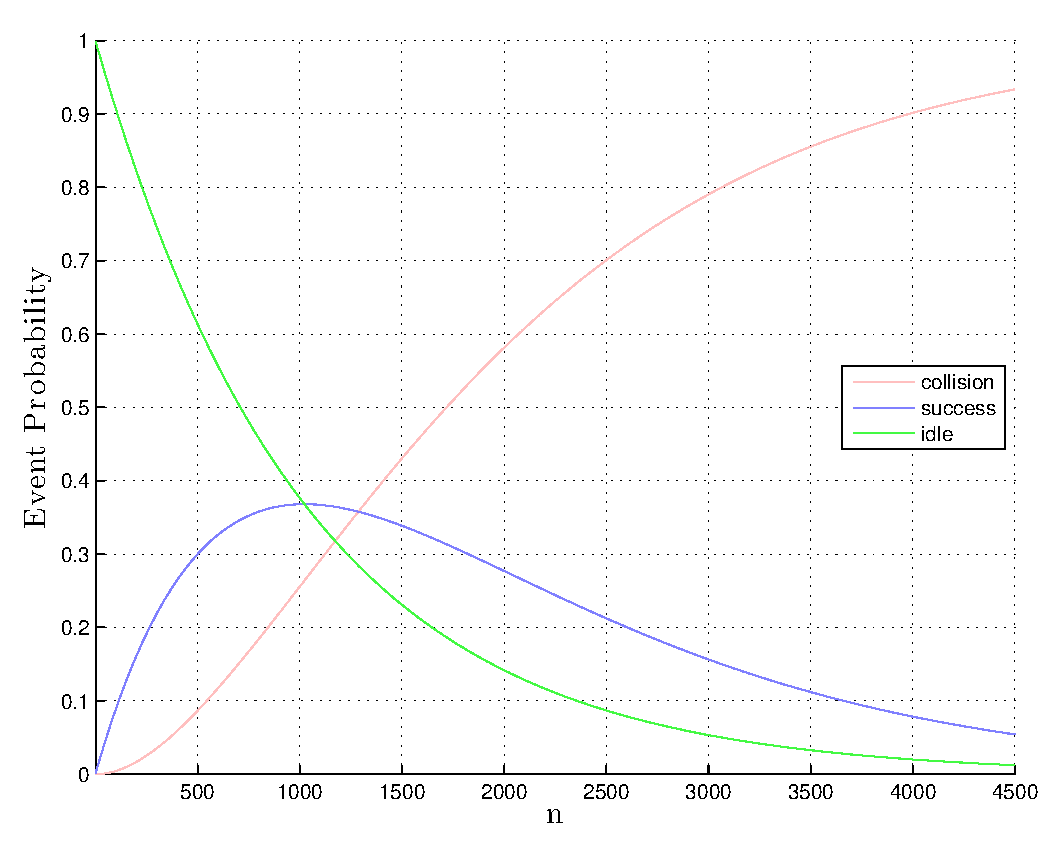
\includegraphics[width=0.7\textwidth]{matlab/Greenberg_MLE/draw_coll_idle_succ_fixed_p}
\caption[\emph{Basic Greenberg}: Event probability fixed $p$]{Probability of \emph{idle}, \emph{successful} or \emph{collided} slots varying $n$ while  $p=1/1024$.  $q_{0}(p,n) \approx  q_{1}(p,n)$ for $n=1023$}
\end{center}
\end{figure}

It is quite immediate to see that:
\begin{itemize}
\item $q_{0}(p,n) \approx q_{1}(p,n)$ when $p\approx {\displaystyle\frac{1}{n}}$ and, obviously,
\item $q_{0}(p,n) \gg q_{1}(p,n)$ and $q_{0}(p,n) \gg q_{2+}(p,n)$ when $p \ll {\displaystyle\frac{1}{n}}$,
\item $q_{2+}(p,n) \gg q_{0}(p,n)$ and $q_{2+}(p,n) \gg q_{0}(p,n)$ when $p \gg {\displaystyle\frac{1}{n}}$.
\end{itemize}
$q_{2+}(p,n)$ is strictly increasing monotonic while $q_{0}(p,n)$ is strictly decreasing. Repeating a large number $T$ of test transmission with  probability $p$ each, we can simply use the number of collisions or idle slots to uniquely determined the batch size. On the other hand, successful probability $q_{1}(p,n)$ is non-monotonic and hence can not be used to uniquely determine the batch size.\\
 
 The proposed technique to refine the estimate is the following.\\
 Running \emph{Basic Greenberg Algorithm} provides a raw estimate and the associated transmission probability $p$. Then we perform $T$ more transmissions and use a \emph{Maximum Likelihood Estimation (MLE)} to refine the estimate.\\ 
 
 Let $T$ be a number of slots of our choice and $N_{0}$, $N_{1}$, $N_{2+}$ random variables which represent the number of time slots with no transmissions, one transmission and collisions respectively.\\
 $N_{0}$, $N_{1}$, $N_{2+}$ are respectively binomial distributions with parameters $B(n,q_{0}(p,n))$, $B(n,q_{1}(p,n))$ and $B(n,q_{2+}(p,n))$. Of course $N_{0}+N_{1}+N_{2+}=T$ and
 \begin{eqnarray*}
E[N_{0}] &=& Tq_{0}(p,n),\\
E[N_{1}] &=& Tq_{1}(p,n),\\
E[N_{2+}] &=& Tq_{2+}(p,n).
\end{eqnarray*}
Let $f_{T}(i,s,c,p',n')$ denote the probability to get $i$ idle, $s$ success and
 $c$ collision slots \begin{align}
f_{T}(i,s,c,p',n')&= \textrm{Pr}(N_{0}=i,N_{1}=s,N_{2+}=c|n=n',p=p')\\
\nonumber
 &=\textrm{Pr}(N_{0}=i|n=n',p=p')\textrm{Pr}(N_{1}=s,N_{2+}=c|n=n'-i,p=p'),
\end{align}
when we transmit with probability $p'$ and considered batch size is $n'$.\\
Let $\mathcal{N}$ be the set of our considered batch sizes, then we can compute
\begin{equation}
MLE(i,s,c,l)=\argmax_{\displaystyle{n' \in \mathcal{N}}} \Bigl( f_{T}\bigl(i,s,c,p(l),n')\cdot \fg\bigl(n',l\bigr)\Bigr).
\label{eq:MLEiscl}
\end{equation}
$MLE(i,s,c,l)$ is a $T \times T \times L$ matrix where $L$ is the maximum slot that can be visited during \emph{Basic Greenberg Algorithm}. $L$ depends on the maximum cardinality  $n_{max}$ considered for the problem. Consequently  $L$ must be chosen so not to worse the performance of our estimator (if $n_{max}$ is smaller than the real batch size $n$) and not to waste too much memory. Setting $L= L(n_{max}) = \lceil\log_{2}n_{max}\rceil$ is a good practical choice, where $\displaystyle n_{max}= \mymax_{n' \in \mathcal{N}}{n'}$.\\
Hence, our estimate is simply the result of a look-up in the $MLE$ table,
\begin{equation}
\hat{n} \longleftarrow MLE(i,s,c,l)
\end{equation}
Is it worth to mention that:
\begin{itemize}
\item  The $MLE$ table must be precomputed before running the estimate algorithm. The computational cost to fill the $MLE$ table depends on $|\mathcal{N}|$ and $L$ and, even if in general the cost is really reasonable, it does not allow for real-time computation.
\item The size of the $MLE$ table does not depend on $|\mathcal{N}|$ but only on $T$ and $L$.
\item The estimate deeply depends on the way the elements in $\mathcal{N}$ are chosen. \\
\end{itemize}

The high level pseudo-code of the algorithm is the following: 
\begin{algorithm}[H]
\begin{algorithmic}
\STATE precompute or load the $MLE$ table characterized by $T$, $L$, $\mathcal{N}$
\STATE $l\gets 0$
\REPEAT
	\STATE $l\gets l+1$
	\STATE $p \gets {\displaystyle\frac{1}{2^{l}}}$
	\STATE choose to transmit with probability $p$
\UNTIL {no collision occurs}
\STATE $(i,s,c) \gets$ events resulting from $T$ transmissions with probability $p$
\STATE $\hat{n}\gets MLE(i,s,c,l)$
\end{algorithmic}
\caption{\algname{EGA $(\mathcal{B},T,\mathcal{N})$}}
\label{alg-greenberg+MLE}
\end{algorithm}
Expected Running time is $\log_{2}n+T$.\\ 
Once both the batch size $n$ and the $MLE$ table are fixed, the probability to estimate $\hat{n}$ can be expressed as:
\begin{equation}
\textrm{Pr}(\hat{n}=n'|n)=\sum_{l}f(n,l)\sum_{i}\sum_{s} \hat{X}_{MLE(i,s,c,l)}(n') \cdot f_{T}\big(i,s,c,p(l),n\bigl),
\end{equation}
 where  $\hat{X}_{MLE(i,s,c,l)}(n')=1$ iff $MLE(i,s,c,l)=n'$,  $\hat{X}_{MLE(i,s,c,l)}(n')=0$ otherwise. \\

DA COMPLETARE
\begin{figure}[H]
\begin{center}
\includegraphics[width=0.7\textwidth]{matlab/Greenberg_MLE/greenberg-mle-T10}
\caption{\emph{EGA}: PROVVISORIO $T=10$  power of 2 distribution.}
\end{center}
\end{figure}

\begin{figure}[H]
\begin{center}
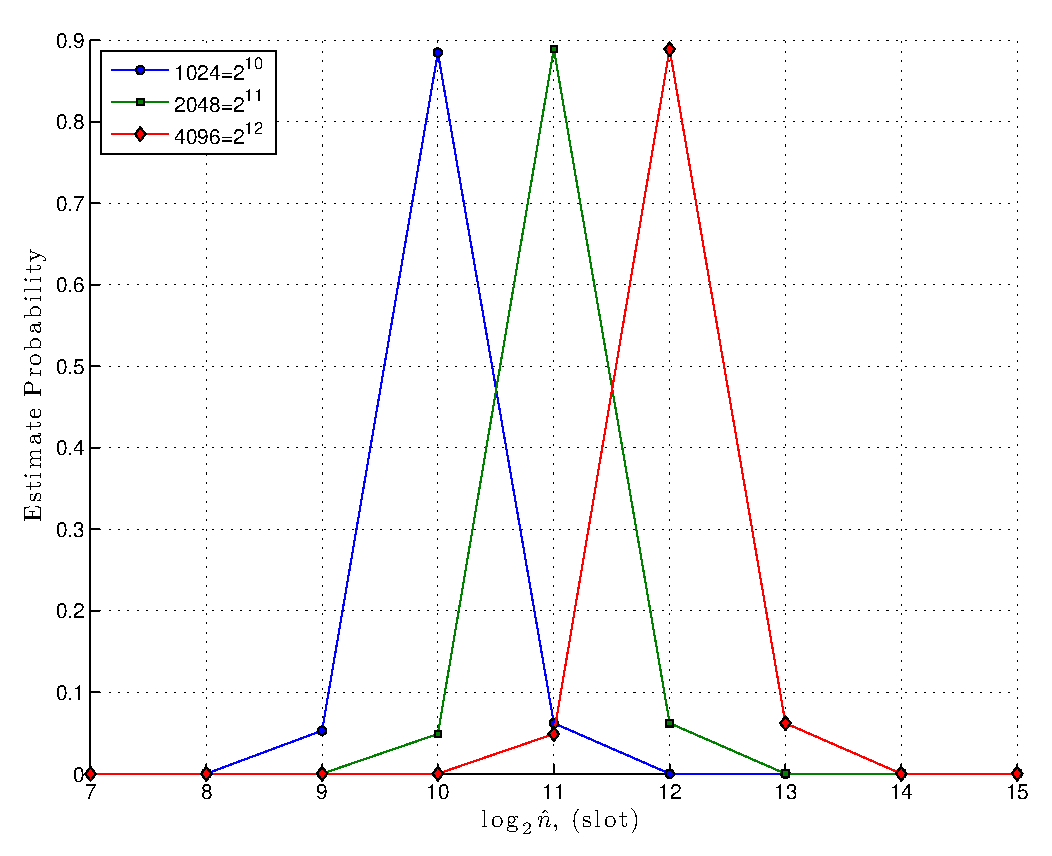
\includegraphics[width=0.7\textwidth]{matlab/Greenberg_MLE/greenberg-mle-T20}
\caption{\emph{EGA}: PROVVISORIO $T=20$  power of 2 distribution.}
\end{center}
\end{figure}

\begin{figure}[H]
\begin{center}
\includegraphics[width=0.7\textwidth]{matlab/Greenberg_MLE/greenberg-mle-T30}
\caption{\emph{EGA}: PROVVISORIO $T=30$  power of 2 distribution.}
\end{center}
\end{figure}

\section{GEGA BSE}
The  \emph{Generalized Enhached Greenberg Algorithm (GEGA)} is a less restrictive form of the EGA algorithm in the sense that we do not \emph{a-priori} limit the possible estimates. This can be simply achieved by letting $\mathcal{N}$ be the set of all the positive integer numbers.
\begin{equation*}
\mathcal{N}=\{1,2,3,...\}
\end{equation*}
In this case the algorithm can be interpreted as follows:
\begin{enumerate}
\item Find the transmission probability $p$ for which the batch size is about 1 node with very high probability,
\item Use $T$ consecutive slots (a ``window'') to refine the estimate. The idea is similar to a window based estimate except that a node is allowed to transmit in each slot.
\end{enumerate}

\noindent Recalling equation \eqref{eq:MLEiscl}, given $i$, $s$, $c$ and $l$, the estimate can be found by solving:
\begin{equation}
\frac{d\Bigl( f_{T}\bigl(i,s,c,p(l),n)\cdot \fg\bigl(n,l\bigr)\Bigr)}{dn}=0,
\end{equation}
which is not trivial to solve and involves numerical problems since $\fg(n,l)$ can present very small product terms. Then we solved the problem by investigating \eqref{eq:MLEiscl} using bisection method and taking the smallest integer $n$ for which
\begin{equation}
f_{T}\bigl(i,s,c,p(l),n+1)\cdot \fg\bigl(n+1,l\bigr)-f_{T}\bigl(i,s,c,p(l),n)\cdot \fg\bigl(n,l\bigr)\leq0.
\end{equation}
As example, the results of this computation when $T=10$ and $l=10$ are presented in Table \ref{tb:GEGA-T10-l10}.

\begin{table}[htbp]
\centering
\resizebox{0.8\textwidth}{!}{
\begin{tabular}{|r|l|l|l|l|l|l|l|l|l|l|l|}
\hline
\backslashbox{$c$}{$s$} & \multicolumn{1}{r|}{0} & \multicolumn{1}{r|}{1} & \multicolumn{1}{r|}{2} & \multicolumn{1}{r|}{3} & \multicolumn{1}{r|}{4} & \multicolumn{1}{r|}{5} & \multicolumn{1}{r|}{6} & \multicolumn{1}{r|}{7} & \multicolumn{1}{r|}{8} & \multicolumn{1}{r|}{9} & \multicolumn{1}{r|}{10} \\ \hline
0 & 352 & 413 & 477 & 545 & 616 & 689 & 765 & 843 & 922 & 1003 & 1086 \\ \hline
1 & 489 & 559 & 632 & 709 & 787 & 868 & 951 & 1036 & 1122 & 1210 & - \\ \hline
2 & 650 & 730 & 812 & 896 & 983 & 1072 & 1162 & 1254 & 1347 & - & - \\ \hline
3 & 838 & 927 & 1017 & 1111 & 1206 & 1302 & 1401 & 1501 & - & - & - \\ \hline
4 & 1055 & 1153 & 1254 & 1356 & 1461 & 1567 & 1675 & - & - & - & - \\ \hline
5 & 1307 & 1416 & 1527 & 1641 & 1757 & 1875 & - & - & - & - & - \\ \hline
6 & 1603 & 1726 & 1851 & 1979 & 2110 & - & - & - & - & - & - \\ \hline
7 & 1962 & 2103 & 2248 & 2396 & - & - & - & - & - & - & - \\ \hline
8 & 2416 & 2585 & 2761 & - & - & - & - & - & - & - & - \\ \hline
9 & 3044 & 3267 & - & - & - & - & - & - & - & - & - \\ \hline
10 & 4111 & - & - & - & - & - & - & - & - & - & - \\ \hline
\end{tabular}
}
\caption{\emph{GEGA}: Possible estimates when $T=10$ and $l=10$}
\label{tb:GEGA-T10-l10}
\end{table}

Looking at the Table \ref{tb:GEGA-T10-l10} emerges that the estimate is always finite. This is good propriety which follows from the bounded moments of the Greenberg algorithm. In general (see Table \ref{tb:window-estimate}), simple window based MLE estimators can not achieve finite estimate when all the events are collisions.\\

The EGA MLE Table can be obtained as sub-case from the GEGA Table considering the largest allowed estimate value lower than and the smallest one larger than the estimate provided by the GEGA algorithm. The EGA estimate will be the one between the two for which the probability in \eqref{eq:MLEiscl} is maximized.\\

\begin{figure}[H]
\begin{center}
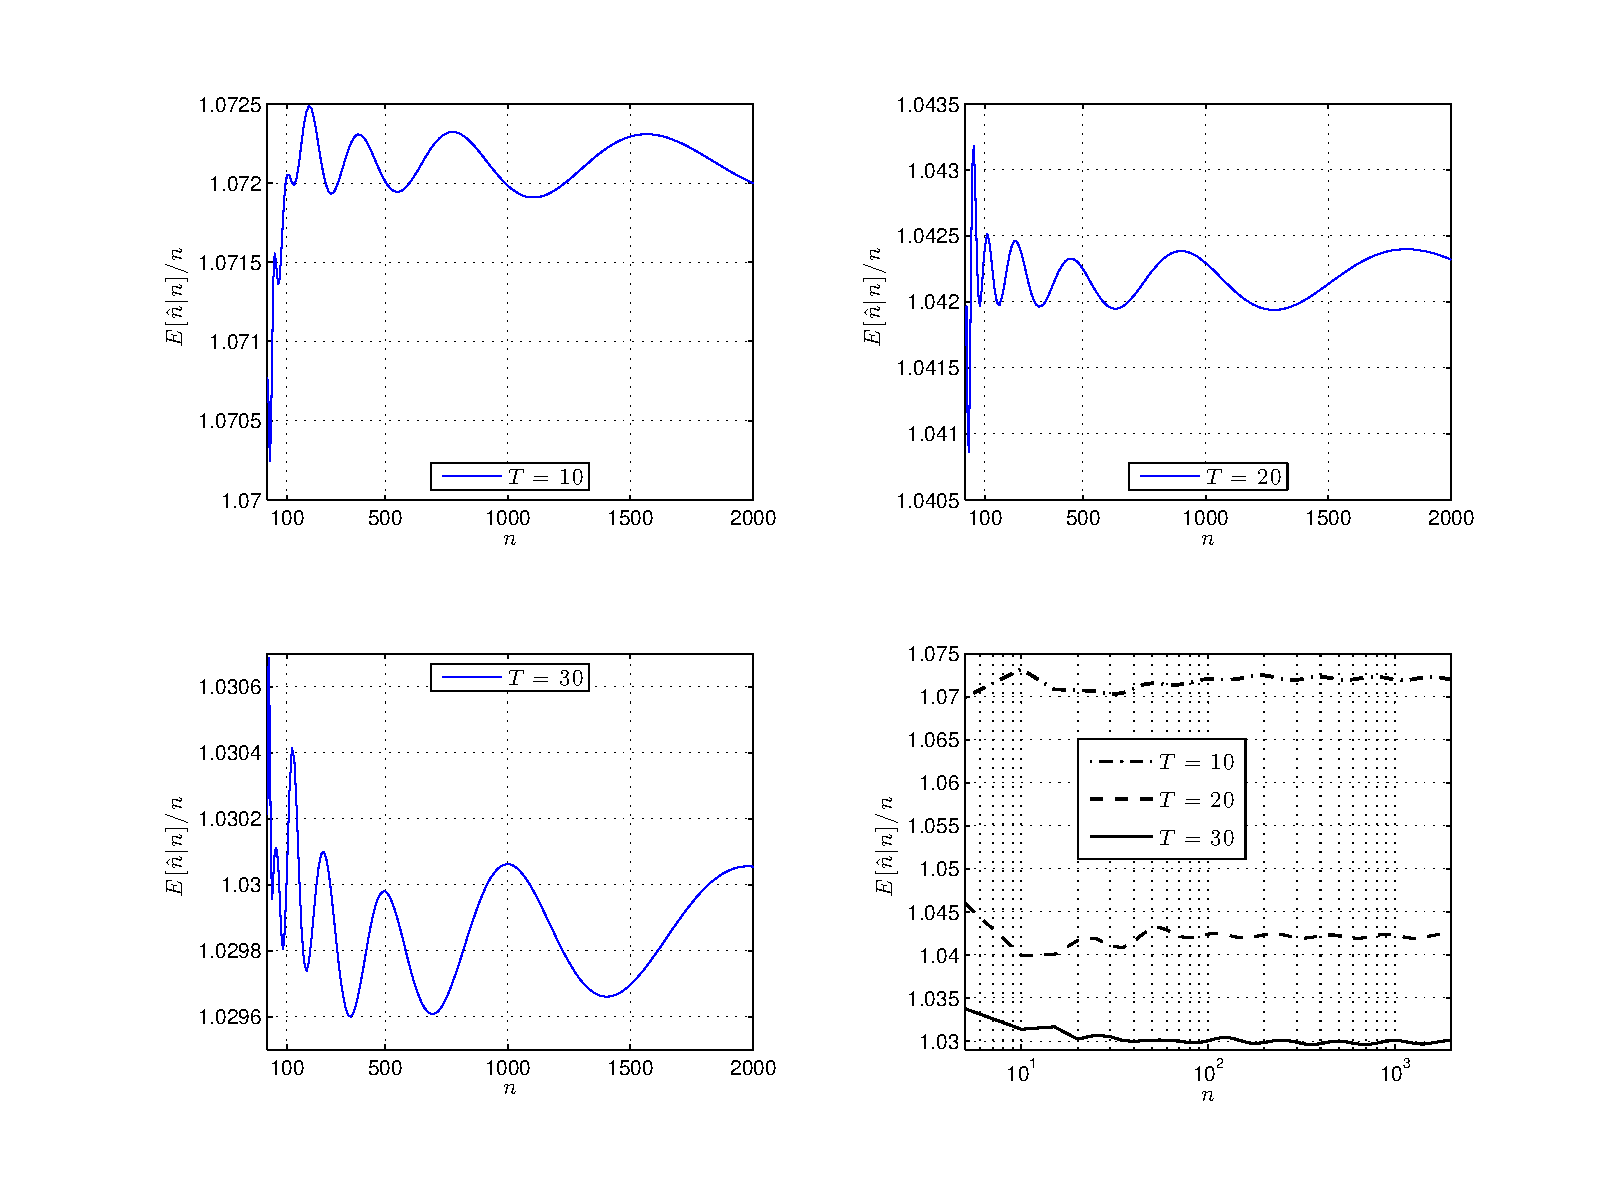
\includegraphics[width=\textwidth]{matlab/GEGA/GEGA-bias-varying-T}
\caption[\emph{GEGA}: Estimate Bias]{\emph{GEGA}: Estimate Bias. The tree plots show the estimate expected value over the real batch size for different $T$.}
\label{fg:GEGA-bias}
\end{center}
\end{figure}

The estimate provided by GEGA showed to be biased. Figure \ref{fg:GEGA-bias} shows that the algorithm tends to overestimate the real batch size. Anyway, the bias can be easily corrected since it is always really near to the average value: the oscillations have really small amplitude. Increasing $T$ reduces the bias as well as the oscillations amplitude. Very small batch sizes (less than 20) show higher oscillations compared to larger ones: this is fact is quite negligible in practice since the oscillations are too small to affect the estimate and are overwhelmed by the rounding operation.  
\chapter{Comparison}
\section{Conclusions}
\label{ch:Comparison}







\begin{comment}

\begin{sidewaystable}
\centering
\begin{tabular}{|llllllllp{1in}lp{1in}|}
\hline
Context   &Length   &Breadth/   &Depth   &Profile   &Pottery   &Flint   &Animal   &Stone   &Other    &C14 Dates \\
  &         &Diameter   &        &          &          &        & 
Bones&&&\\
\hline
&&&&&&&&&&\\
\multicolumn{10}{|l}{\bf Grooved Ware}&\\
784 &---   &0.90m &0.18m &Sloping U &P1    &$\times$46  &  $\times$8  &&$\times$2 bone&  2150$\pm$ 100 BC\\
785 &---   &1.00m &0.12  &Sloping U &P2--4 &$\times$23  &  $\times$21 & Hammerstone &---&---\\
962 &---   &1.37m &0.20m &Sloping U &P5--6 &$\times$48  &  $\times$57* & ---&     ---&1990 $\pm$ 80 BC (Layer 4) 1870 $\pm$90 BC (Layer 1)\\
983 &0.83m &0.73m &0.25m &Stepped U &---   &$\times$18  &  $\times$8 & ---& Fired clay&---\\
&&&&&&&&&&\\
\multicolumn{10}{|l}{\bf Beaker}&\\
552 &---   &0.68m &0.12m &Saucer    &P7--14 &---        & --- & --- &--- &---\\
790 &---   &0.60m &0.25m &U         &P15    &$\times$12 & --- & Quartzite-lump&--- &---\\
794 &2.89m &0.75m &0.25m &Irreg.    &P16    $\times$3   & --- & --- &--- &---\\
\hline
\end{tabular}
 
\caption[Grooved Ware and Beaker Features, their Finds and Radiocarbon
Dates]{Grooved Ware and Beaker Features, their Finds and Radiocarbon
Dates; For a breakdown of the Pottery Assemblages see Tables I and
III; for the Flints see Tables II and IV; for the Animal Bones see
Table V.}\label{rotfloat2} \end{sidewaystable} 
\end{comment}

\begin{appendices}

\chapter[Appendix]{}

\section{Probability}
\textcolor{red}{sezione provvisoria}
\subsection{Chebyshev's inequality}
Let $X$ be a \emph{random variable} with expected value $\mu$ and finite variance $\sigma^{2}$. Then for any real number $k>0$,
\begin{equation}
\Pr(\left|X-\mu\right|\geq k)\leq\frac{\sigma^{2}}{k^2}
\label{eq:cheby}
\end{equation}
\subsection{Binomial Distribution}

$B(n,p)$
\subsubsection{Poisson Approximation}
The binomial distribution converges towards the Poisson distribution as the number of trials goes to infinity while the product $np$ remains fixed. Therefore the Poisson distribution with parameter $\lambda = np$ can be used as an approximation to $B(n, p)$ of the binomial distribution if $n$ is sufficiently large and $p$ is sufficiently small. According to two rules of thumb, this approximation is good if $n \geq 20$ and $p \leq 0.05$, or if $n \geq 100$ and $np \leq 10$.
\subsubsection{Normal Approximation}
If $n$ is large enough, then the skew of the distribution is not too great. In this case, if a suitable continuity correction is used, then an excellent approximation to $B(n, p)$ is given by the normal distribution $\mathcal{N}(np,np(1-p))$\\
The approximation generally improves as $n$ increases and is better when $p$ is not near to 0 or 1. Various rules of thumb may be used to decide whether $n$ is large enough, and $p$ is far enough from the extremes of zero or unity:
One rule is that both $n p$ and $n(1-p)$ must be greater than 5. However, the specific number varies from source to source, and depends on how good an approximation one wants; some sources give 10.\\

oppure dal libro $np(1-p)\geq 10$.




\subsection{Poisson Distribution}
\subsection{Normal Distribution}
 $\mathcal{N}(\mu,\sigma^{2})$
\begin{equation}
f(x)= \frac{1}{\sqrt{2\pi\sigma^{2}}}\exp{-\frac{(x-\mu)^{2}}{2\sigma^{2}}}
\end{equation}

\section{Greenberg bounded \emph{m}-moments}

In general for base $b$ greenberg algorithm the first and second moments are bounded by:

\begin{equation}
\phi(b)= \frac{1}{\log b} \int_{0}^{\infty} \! e^{-x}(1+x) \prod_{k=1}^{\infty}(1-e^{-b^{k}x}(1+b^{k}x))x^{-2} \, dx
\end{equation}

\begin{equation}
\Phi(b)= \frac{1}{\log b} \int_{0}^{\infty} \! e^{-x}(1+x) \prod_{k=1}^{\infty}(1-e^{-b^{k}x}(1+b^{k}x))x^{-3} \, dx
\end{equation}

\textcolor{red}{note sul calcolo\\ va velocemente a 0 quind basta considerare un intervallo iniziale  limitato\\
anche per produttoria con k è lo stesso.\\ risolto con quad matlab}

\section{CBT Estimate Experimental Distribution}

Following tables \ref{CBT-table-1} shows the behavior of CBT Algorithm (section \ref{cbt-estimation}) for estimation.  Simulation was implemented in matlab.
The resulting distribution of $\hat{n}$ fixed $n$ is the result of averaging \numprint{100000} runs of CBT Algorihm applied on uniformly random generated nodes ID batches.\\ 

\begin{table}[H]
\caption[Experimentally computed CBT Estimate Distributon]{Experimentally computed CBT Estimate Distributon. Table 1/3}
\label{CBT-table-1}
\resizebox{\textwidth}{!}{
\begin{tabular}{r|cccccccccccc}
n&$\hat{n}:$&2&4&8&16&32&64&128&256&512&1024&2048 \\\hline

2 &&0.499 &0.253 &0.125 &0.061 &0.031 &0.015 &0.007 &0.004 &0.002 &9e-04 &4e-04\\\hline

4 &&&0.189 &0.303 &0.225 &0.133 &0.072 &0.038 &0.020 &0.010 &0.005 &0.002\\\hline

8 &&&0.055 &0.212 &0.261 &0.201 &0.126 &0.071 &0.037 &0.019 &0.009 &0.005\\\hline

16 &&&8e-04 &0.070 &0.209 &0.252 &0.197 &0.125 &0.070 &0.038 &0.019 &0.010\\\hline

32 &&&&0.003 &0.075 &0.213 &0.249 &0.195 &0.123 &0.069 &0.037 &0.018\\\hline

64 &&&&&0.004 &0.077 &0.208 &0.250 &0.193 &0.124 &0.069 &0.037\\\hline

128 &&&&&&0.005 &0.081 &0.208 &0.247 &0.191 &0.123 &0.069\\\hline

256 &&&&&&2e-05 &0.006 &0.079 &0.209 &0.246 &0.193 &0.123\\\hline

512 &&&&&&&&0.005 &0.081 &0.207 &0.245 &0.193\\\hline

1024 &&&&&&&&&0.005 &0.080 &0.208 &0.245\\\hline

2048 &&&&&&&&&2e-05 &0.005 &0.080 &0.209\\\hline

4096 &&&&&&&&&&1e-05 &0.006 &0.082\\\hline

8192 &&&&&&&&&&&1e-05 &0.006\\\hline

16384 &&&&&&&&&&&&2e-05\\\hline

32768 &&&&&&&&&&&&\\\hline

\end{tabular}
}

\end{table}
\begin{table}[H]
\ContinuedFloat
\caption[]{Experimentally computed CBT Estimate Distributon. Table 2/3}
\resizebox{\textwidth}{!}{
\begin{tabular}{r|cccccccccccc}
n&$\hat{n}:$&4096&8192&16384&32768&$2^{16}$&$2^{17}$&$2^{18}$&$2^{19}$&$2^{20}$&$2^{21}$&$2^{22}$ \\\hline

2 &&2e-04 &1e-04 &1e-04 &&&&1e-05 &&&&\\\hline

4 &&0.001 &5e-04 &3e-04 &1e-04 &6e-05 &4e-05 &&2e-05 &1e-05 &&\\\hline

8 &&0.002 &0.001 &6e-04 &3e-04 &9e-05 &8e-05 &4e-05 &1e-05 &&&\\\hline

16 &&0.005 &0.003 &0.001 &6e-04 &3e-04 &2e-04 &6e-05 &2e-05 &2e-05 &&\\\hline

32 &&0.009 &0.005 &0.003 &0.001 &6e-04 &3e-04 &1e-04 &1e-04 &6e-05 &1e-05 &1e-05\\\hline

64 &&0.019 &0.009 &0.005 &0.002 &0.001 &7e-04 &3e-04 &7e-05 &4e-05 &&2e-05\\\hline

128 &&0.037 &0.019 &0.010 &0.005 &0.003 &0.001 &5e-04 &4e-04 &2e-04 &5e-05 &4e-05\\\hline

256 &&0.068 &0.038 &0.019 &0.009 &0.005 &0.002 &0.001 &6e-04 &3e-04 &6e-05 &8e-05\\\hline

512 &&0.123 &0.071 &0.037 &0.019 &0.010 &0.005 &0.002 &0.001 &6e-04 &3e-04 &2e-04\\\hline

1024 &&0.193 &0.122 &0.070 &0.037 &0.019 &0.010 &0.005 &0.002 &0.001 &6e-04 &2e-04\\\hline

2048 &&0.246 &0.194 &0.123 &0.068 &0.037 &0.019 &0.010 &0.005 &0.002 &0.001 &6e-04\\\hline

4096 &&0.210 &0.246 &0.193 &0.121 &0.068 &0.037 &0.019 &0.009 &0.004 &0.003 &0.001\\\hline

8192 &&0.080 &0.208 &0.247 &0.192 &0.123 &0.070 &0.037 &0.019 &0.009 &0.005 &0.002\\\hline

16384 &&0.006 &0.080 &0.208 &0.247 &0.192 &0.123 &0.069 &0.037 &0.019 &0.010 &0.005\\\hline

32768 &&&0.006 &0.079 &0.209 &0.248 &0.194 &0.122 &0.069 &0.036 &0.019 &0.010\\\hline

\end{tabular}
}

\end{table}
\begin{table}[H]\ContinuedFloat
\caption[]{Experimentally computed CBT Estimate Distributon. Table 3/3}
\resizebox{\textwidth}{!}{
\begin{tabular}{r|ccccccccccc}
n&$\hat{n}:$&$2^{23}$&$2^{24}$&$2^{25}$&$2^{26}$&$2^{27}$&$2^{28}$&$2^{29}$&$2^{30}$&$2^{31}$&$2^{32}$ \\\hline

2 &&&&&&&&&&&\\\hline

4 &&&&&&&&&&&\\\hline

8 &&&&&&&&&&&\\\hline

16 &&&&&&&&&&&\\\hline

32 &&1e-05 &&&&&&&&&\\\hline

64 &&2e-05 &&&&1e-05 &&&&&\\\hline

128 &&4e-05 &&1e-05 &&&&&&&\\\hline

256 &&4e-05 &1e-05 &&2e-05 &&&1e-05 &&&\\\hline

512 &&7e-05 &2e-05 &1e-05 &3e-05 &1e-05 &&&&&\\\hline

1024 &&2e-04 &1e-04 &4e-05 &&2e-05 &1e-05 &&&&\\\hline

2048 &&3e-04 &1e-04 &3e-05 &3e-05 &3e-05 &3e-05 &&&&\\\hline

4096 &&6e-04 &3e-04 &9e-05 &7e-05 &1e-05 &&&&&\\\hline

8192 &&0.001 &8e-04 &3e-04 &2e-04 &8e-05 &7e-05 &2e-05 &3e-05 &1e-05 &\\\hline

16384 &&0.002 &0.001 &6e-04 &3e-04 &1e-04 &1e-04 &4e-05 &&&\\\hline

32768 &&0.005 &0.002 &0.001 &6e-04 &3e-04 &2e-04 &1e-04 &1e-05 &2e-05 &1e-05\\\hline

\end{tabular}
}
\end{table}

\lstinputlisting{matlab/CBT/cbtsimpletest.m}
\lstinputlisting{matlab/CBT/cbtsplit.m}
\lstinputlisting{matlab/CBT/cbtfulltest.m}
%\verbatiminput{matlab/CBT/cbtfulltest.m}

\section{Greenberg Estimate Distribution}
In following table \ref{basic-greenberg-stop-probabilities} we report how the end  up probability (equation \ref{eq:bgstopprobability}) is distributed among slots given a batch of size $n$.  Column ``$n$'' lists  the considered batch sizes. $\hat{n}$ is the resulting estimation (without corrections) when ending up in the underneath slot.\\  For sake of simplicity considered values are all powers of 2.\\
Datas presented were post-processed to become more accessible:
\begin{itemize}
\item values above $10^{-3}$ are reported in format ('\emph{\%1.3f}');
\item values below $10^{-12}$ are not presented since are tight close to 0.
\item other values are presented in exponential notation and rounded to the first meaningful digit ('\emph{\%1.e}')
\end{itemize}


\begin{sidewaystable}
%%%%%
\flushleft
\resizebox{25cm}{!}{
\begin{tabular}{r|ccccccccccccccccccccccc}
&$\hat{n}$& 2 &4 &8 &16 &32 &64 &128 &256 &512 &1024 &2048 &4096 &8192 &16384 &32768 &65536\\
n & slot:& 1 &2 &3 &4 &5 &6 &7 &8 &9 &10 &11 &12 &13 &14 &15 & 16\\ 
\toprule
1 &&1.000 &&&&&&&&&\\\hline

2 &&0.750 &0.234 &0.015 &2e-04 &1e-06 &9e-10 &&&&&&&&\\\hline

4 &&0.312 &0.508 &0.166 &0.014 &3e-04 &2e-06 &2e-09 &&&&&&&\\\hline

8 &&0.035 &0.354 &0.450 &0.147 &0.013 &3e-04 &2e-06 &4e-09 &1e-12 &&&&&&\\\hline

16 &&3e-04 &0.063 &0.363 &0.422 &0.138 &0.013 &3e-04 &2e-06 &4e-09 &2e-12 &&&&&\\\hline

32 &&8e-09 &0.001 &0.078 &0.366 &0.409 &0.134 &0.013 &3e-04 &2e-06 &4e-09 &2e-12 &&&&\\\hline

64 &&&2e-07 &0.002 &0.084 &0.367 &0.402 &0.131 &0.013 &3e-04 &2e-06 &4e-09 &2e-12 &&&\\\hline

128 &&&&7e-07 &0.002 &0.088 &0.367 &0.399 &0.130 &0.013 &3e-04 &2e-06 &5e-09 &2e-12 &&\\\hline

256 &&&&&1e-06 &0.003 &0.090 &0.368 &0.397 &0.130 &0.013 &3e-04 &2e-06 &5e-09 &2e-12 & \\\hline

512 &&&&&&2e-06 &0.003 &0.090 &0.368 &0.397 &0.130 &0.012 &3e-04 &2e-06 &5e-09 &2e-12 \\\hline
1024 &&&&&&&2e-06 &0.003 &0.091 &0.368 &0.396 &0.129 &0.012 &3e-04 &2e-06 &5e-09 &2e-12 \\
\bottomrule
\end{tabular}
}

\begin{tabular}{c}
\\
\end{tabular}
\resizebox{25cm}{!}{
\begin{tabular}{r|ccccccccccccccccccccccc}
&$\hat{n}$&128 &256 &512 &1024 &2048 &4096 &8192 &16384 &32768 &65536 &$2^{17}$ &$2^{18}$ &$2^{19}$ &$2^{20}$ &$2^{21}$ &$2^{22}$ \\ 
n & slot:& 7 &8 &9 &10 &11 &12 &13 &14 &15 &16 &17 &18 &19 &20 &21 &22 \\ 
\toprule


2048 &&2e-06 &0.003 &0.091 &0.368 &0.396 &0.129 &0.012 &3e-04 &2e-06 &5e-09 &2e-12 &&&&&\\\hline

4096 &&&2e-06 &0.003 &0.091 &0.368 &0.396 &0.129 &0.012 &3e-04 &2e-06 &5e-09 &2e-12 &&&&\\\hline

8192 &&&&2e-06 &0.003 &0.091 &0.368 &0.396 &0.129 &0.012 &3e-04 &2e-06 &5e-09 &2e-12 &&&\\\hline

16384 &&&&&2e-06 &0.003 &0.091 &0.368 &0.396 &0.129 &0.012 &3e-04 &2e-06 &5e-09 &2e-12 &&\\\hline

32768 &&&&&&2e-06 &0.003 &0.091 &0.368 &0.396 &0.129 &0.012 &3e-04 &2e-06 &5e-09 &2e-12 &\\\hline

65536 &&&&&&&2e-06 &0.003 &0.091 &0.368 &0.396 &0.129 &0.012 &3e-04 &2e-06 &5e-09 &2e-12\\

\bottomrule
\end{tabular}
}
%%%%
\caption{Analytically computed basic Greeenberg Estimate Distribution}
\label{basic-greenberg-stop-probabilities}

\end{sidewaystable}

\end{appendices}


\begin{thebibliography}{99}
 
\bibitem{popovski}
  Peter Popovski, Frank H.P. Fitzek, Ramjee Prasad, \emph{ A Class of Algorithms for Collision Resolution with Multiplicity Estimation}, Springer, Algorithmica, Vol. 49, No. 4, December 2007, 286-317
  
\bibitem{lucent}
Murali Kodialam, Thyaga Nandagopal, \emph{Fast and Reliable Estimation Schemes in RFID Systems}, MobiCom '06: Proceedings of the 12th annual international conference on Mobile computing and networking, ACM , September 2006, 322-333 
 
\bibitem{cidon}
 Israel Cidon, Moshe Side, \emph{Conflict Multiplicity Estimation and Batch Resolution Algorithms}, IEEE Transactions On Information Theory, Vol. 34, No. 1, January 1988, 101-110
 
\bibitem{greenberg87}
  Albert G. Greenberg, Philippe Flajolet,  Richard E. Ladner,
  \emph{Estimating the Multiplicities of Conflicts to Speed Their Resolution in Multiple Access Channels},
  Journal of the Association for Computing Machinery,
  Vol 34, No. 2, April 1987, 289-325
  
 \bibitem{capetanakis}
  J.I. Capetanakis, \emph{ Tree algorithms for packet broadcast channels}, IEEE Transactions On Information Theory, Vol. 25, No. 5, September 1979, 505-515
 \end{thebibliography}
\end{document}